\documentclass[a4paper,10pt,twoside]{book}
\usepackage{amd}

% %--------------------------------------------------------------------------
% %         General Setting
% %--------------------------------------------------------------------------

\graphicspath{{Images/}{../Images/}} %Path of figures
\setkeys{Gin}{width=0.85\textwidth} %Size of figures
\setlength{\cftbeforechapskip}{3pt} %space between items in toc
\setlength{\parindent}{0.5cm} % Idk
% Theorem System
% The following boxes are provided:
%   Definition:     \defn 
%   Theorem:        \thm 
%   Lemma:          \lem
%   Corollary:      \cor
%   Proposition:    \prop   
%   Claim:          \clm
%   Fact:           \fact
%   Proof:          \pf
%   Example:        \ex
%   Remark:         \rmk (sentence), \rmkb (block)
% Suffix
%   r:              Allow Theorem/Definition to be referenced, e.g. thmr
%   p:              Add a short proof block for Lemma, Corollary, Proposition or Claim, e.g. lemp
%                   For theorems, use \pf for proof blocks

% ======= Real examples : 

% \defn{Definition Name}{
%     A defintion.
% }

% \thmr{Theorem Name}{mybigthm}{
%     A theorem.
% }

% \lem{Lemma Name}{
%     A lemma.
% }

% \fact{
%     A fact.
% }

% \cor{
%     A corollary.
% }

% \prop{
%     A proposition.
% }

% \clmp{}{
%     A claim.
% }{
%     A reference to Theorem~\ref{thm:mybigthm}
% }

% \pf{
%    proof.

% \ex{
%     some examples. 
% }

% \rmk{
%     Some remark.
% }

% \rmkb{
%     Some more remark.
% }

\usepackage{xcolor}

% Define custom colors
\definecolor{defscol}{HTML}{ecd8d7} %For definitions
\definecolor{asumscol}{HTML}{ecd8d7} %For Assumptions

\definecolor{rmkscol}{HTML}{313160} %For remarks
\definecolor{exmscol}{HTML}{e04b52} %For examples

\definecolor{lemscol}{HTML}{2c3943} %For Lemmes
\definecolor{thmscol}{HTML}{595765} %For Theorems
\definecolor{prpscol}{HTML}{9c98b1} %For proposition
\definecolor{corscol}{HTML}{dfd9fd} %For corrolaries

\definecolor{clmscol}{HTML}{165c58} %For claims
\definecolor{facscol}{HTML}{28a8a1} %For facts



% ============================
% Definition
% ============================
\newtcbtheorem[number within=section]{mydefinition}{Definition}
{
    enhanced,
    frame hidden,
    titlerule=0mm,
    toptitle=1mm,
    bottomtitle=1mm,
    fonttitle=\bfseries\large,
    coltitle=black,
    colbacktitle=defscol!40!white,
    colback=defscol!20!white,
}{defn}

\NewDocumentCommand{\defn}{m+m}{
    \begin{mydefinition}{#1}{}
        #2
    \end{mydefinition}
}

\NewDocumentCommand{\defnr}{mm+m}{
    \begin{mydefinition}{#1}{#2}
        #3
    \end{mydefinition}
}

% ============================
% Assumption
% ============================
\newtcbtheorem[use counter from=mydefinition]{myassumption}{Assumption}
{
    enhanced,
    frame hidden,
    titlerule=0mm,
    toptitle=1mm,
    bottomtitle=1mm,
    fonttitle=\bfseries\large,
    coltitle=black,
    colbacktitle=asumscol!40!white,
    colback=asumscol!20!white,
}{asum}

\NewDocumentCommand{\asum}{m+m}{
    \begin{myassumption}{#1}{}
        #2
    \end{myassumption}
}

\NewDocumentCommand{\asumr}{mm+m}{
    \begin{myassumption}{#1}{#2}
        #3
    \end{myassumption}
}

% ============================
% Theorem
% ============================

\newtcbtheorem[use counter from=mydefinition]{mytheorem}{Theorem}
{
    enhanced,
    frame hidden,
    titlerule=0mm,
    toptitle=1mm,
    bottomtitle=1mm,
    fonttitle=\bfseries\large,
    coltitle=black,
    colbacktitle=thmscol!40!white,
    colback=thmscol!20!white,
}{thm}

\NewDocumentCommand{\thm}{m+m}{
    \begin{mytheorem}{#1}{}
        #2
    \end{mytheorem}
}

\NewDocumentCommand{\thmr}{mm+m}{
    \begin{mytheorem}{#1}{#2}
        #3
    \end{mytheorem}
}

\newenvironment{thmpf}{
	{\noindent{\it \textbf{Proof for Theorem.}}}
	\tcolorbox[blanker,breakable,left=5mm,parbox=false,
    before upper={\parindent15pt},
    after skip=10pt,
	borderline west={1mm}{0pt}{thmscol!40!white}]
}{
    \textcolor{thmscol!40!white}{\hbox{}\nobreak\hfill$\blacksquare$} 
    \endtcolorbox
}

\NewDocumentCommand{\thmp}{m+m+m}{
    \begin{mytheorem}{#1}{}
        #2
    \end{mytheorem}

    \begin{thmpf}
        #3
    \end{thmpf}
}

% ============================
% Lemma
% ============================

\newtcbtheorem[use counter from=mydefinition]{mylemma}{Lemma}
{
    enhanced,
    frame hidden,
    titlerule=0mm,
    toptitle=1mm,
    bottomtitle=1mm,
    fonttitle=\bfseries\large,
    coltitle=black,
    colbacktitle=lemscol!40!white,
    colback=lemscol!20!white,
}{lem}

\NewDocumentCommand{\lem}{m+m}{
    \begin{mylemma}{#1}{}
        #2
    \end{mylemma}
}

\newenvironment{lempf}{
	{\noindent{\it \textbf{Proof for Lemma}}}
	\tcolorbox[blanker,breakable,left=5mm,parbox=false,
    before upper={\parindent15pt},
    after skip=10pt,
	borderline west={1mm}{0pt}{lemscol!40!white}]
}{
    \textcolor{lemscol!40!white}{\hbox{}\nobreak\hfill$\blacksquare$} 
    \endtcolorbox
}

\NewDocumentCommand{\lemp}{m+m+m}{
    \begin{mylemma}{#1}{}
        #2
    \end{mylemma}

    \begin{lempf}
        #3
    \end{lempf}
}

% ============================
% Corollary
% ============================

\newtcbtheorem[use counter from=mydefinition]{mycorollary}{Corollary}
{
    enhanced,
    frame hidden,
    titlerule=0mm,
    toptitle=1mm,
    bottomtitle=1mm,
    fonttitle=\bfseries\large,
    coltitle=black,
    colbacktitle=corscol!40!white,
    colback=corscol!20!white,
}{cor}

\NewDocumentCommand{\cor}{+m}{
    \begin{mycorollary}{}{}
        #1
    \end{mycorollary}
}

\newenvironment{corpf}{
	{\noindent{\it \textbf{Proof for Corollary.}}}
	\tcolorbox[blanker,breakable,left=5mm,parbox=false,
    before upper={\parindent15pt},
    after skip=10pt,
	borderline west={1mm}{0pt}{corscol!40!white}]
}{
    \textcolor{corscol!40!white}{\hbox{}\nobreak\hfill$\blacksquare$} 
    \endtcolorbox
}

\NewDocumentCommand{\corp}{m+m+m}{
    \begin{mycorollary}{}{}
        #1
    \end{mycorollary}

    \begin{corpf}
        #2
    \end{corpf}
}

% ============================
% Proposition
% ============================

\newtcbtheorem[use counter from=mydefinition]{myproposition}{Proposition}
{
    enhanced,
    frame hidden,
    titlerule=0mm,
    toptitle=1mm,
    bottomtitle=1mm,
    fonttitle=\bfseries\large,
    coltitle=black,
    colbacktitle=prpscol!30!white,
    colback=prpscol!20!white,
}{prop}

\NewDocumentCommand{\prop}{+m}{
    \begin{myproposition}{}{}
        #1
    \end{myproposition}
}

\newenvironment{proppf}{
	{\noindent{\it \textbf{Proof for Proposition.}}}
	\tcolorbox[blanker,breakable,left=5mm,parbox=false,
    before upper={\parindent15pt},
    after skip=10pt,
	borderline west={1mm}{0pt}{prpscol!40!white}]
}{
    \textcolor{prpscol!40!white}{\hbox{}\nobreak\hfill$\blacksquare$} 
    \endtcolorbox
}



\NewDocumentCommand{\propp}{+m+m}{
    \begin{myproposition}{}{}
        #1
    \end{myproposition}

    \begin{proppf}
        #2
    \end{proppf}
}

% ============================
% Claim
% ============================

\newtcbtheorem[use counter from=mydefinition]{myclaim}{Claim}
{
    enhanced,
    frame hidden,
    titlerule=0mm,
    toptitle=1mm,
    bottomtitle=1mm,
    fonttitle=\bfseries\large,
    coltitle=black,
    colbacktitle=clmscol!40!white,
    colback=clmscol!20!white,
}{clm}

\NewDocumentCommand{\clm}{m+m}{
    \begin{myclaim*}{#1}{}
        #2
    \end{myclaim*}
}

\newenvironment{clmpf}{
	{\noindent{\it \textbf{Proof for Claim.}}}
	\tcolorbox[blanker,breakable,left=5mm,parbox=false,
    before upper={\parindent15pt},
    after skip=10pt,
	borderline west={1mm}{0pt}{clmscol!40!white}]
}{
    \textcolor{clmscol!40!white}{\hbox{}\nobreak\hfill$\blacksquare$} 
    \endtcolorbox
}

\NewDocumentCommand{\clmp}{m+m+m}{
    \begin{myclaim*}{#1}{}
        #2
    \end{myclaim*}

    \begin{clmpf}
        #3
    \end{clmpf}
}

% ============================
% Fact
% ============================

\newtcbtheorem[use counter from=mydefinition]{myfact}{Fact}
{
    enhanced,
    frame hidden,
    titlerule=0mm,
    toptitle=1mm,
    bottomtitle=1mm,
    fonttitle=\bfseries\large,
    coltitle=black,
    colbacktitle=facscol!40!white,
    colback=facscol!20!white,
}{fact}

\NewDocumentCommand{\fact}{+m}{
    \begin{myfact}{}{}
        #1
    \end{myfact}
}

% ============================
% Proof
% ============================

\NewDocumentCommand{\pf}{+m}{
    \begin{proof}
        [\noindent\textbf{Proof.}]
        #1
    \end{proof}
}

% ============================
% Example
% ============================


\newenvironment{myexample}{
    \tcolorbox[blanker,breakable,left=5mm,parbox=false,
    before upper={\parindent15pt},
    after skip=10pt,
	borderline west={1mm}{0pt}{clmscol!40!white}]
}{
    \textcolor{clmscol!40!white}{\hbox{}\nobreak\hfill$\blacksquare$} 
    \endtcolorbox
}

\NewDocumentCommand{\exm}{m+m}{
    \begin{myexample}
	{\noindent{\it \textbf{Example : #1 }}}\\ 
        #2
    \end{myexample}
}


% ============================
% Remark
% ============================


\NewDocumentCommand{\rmk}{+m}{
    {\it \color{rmkscol!40!white}#1}
}

\newenvironment{remark}{
    \par
    \vspace{5pt}
    \begin{minipage}{\textwidth}
        {\par\noindent{\textbf{Remark.}}}
        \tcolorbox[blanker,breakable,left=5mm,
        before skip=10pt,after skip=10pt,
        borderline west={1mm}{0pt}{rmkscol!20!white}]
}{
        \endtcolorbox
    \end{minipage}
    \vspace{5pt}
}

\NewDocumentCommand{\rmkb}{+m}{
    \begin{remark}
        #1
    \end{remark}
}













% % Old styles hh 

% %--------------------------------------------------------------------------
% % 		THEOREMES STYLE
% %--------------------------------------------------------------------------

% %-------		DEFINITION 		-------	
% \newcounter{defo}[chapter]
% \newenvironment{defi}[1]{\refstepcounter{defo} 
% \begin{tcolorbox}[colback=yellow!20!white,colframe=yellow!15!black,title= \textbf{Définition \thechapter \ $\blacklozenge$ \thedefo \ | #1}]}{\end{tcolorbox}}

% %-------		THEOREME 		-------	
% \newcounter{th}[chapter]
% \newenvironment{thm}[1]{\refstepcounter{th}
% \begin{tcolorbox}[colback=mycolor!10,colframe=mycolor!10!black!80,title=\textbf{ Théorème \thechapter \ $\blacklozenge$ \theth \ | #1}]}{\end{tcolorbox}}

% %-------		PROPOSITION 		-------	
% \newcounter{prop}[chapter]
% \newenvironment{propt}[1]{\refstepcounter{prop}
% \begin{tcolorbox}[colback=mycolor!5,colframe=mycolor!10!linkscolor!80 ,title=\textbf{ Proposition \thechapter \ $\blacklozenge$ \theprop \ | #1}]}{\end{tcolorbox}}

% %-------		COROLLAIRE		-------
% \newcounter{cor}[chapter]
% \newenvironment{corr}[1]{\refstepcounter{cor}
% \begin{tcolorbox}[colback=mycolor!2,colframe=mycolor!10!linkscolor!40 ,title= Corolaire \thechapter \ $\blacklozenge$ \thecor \ | #1]}{\end{tcolorbox}}

% %-------		LEMME			-------
% \newcounter{lem}[chapter]
% \newenvironment{lemme}[1]{\refstepcounter{lem}
% \begin{tcolorbox}[colback=mycolor!10!blue!2,colframe=mycolor!50!blue!30,title=\textbf{Lemme \thechapter \ $\blacklozenge$ \thelem \ | #1}]}{\end{tcolorbox}}

% %-------		METHODE 			-------
% \newcounter{met}[chapter]
% \newenvironment{meth}[1]{\refstepcounter{met}
% \begin{tcolorbox}
% [enhanced jigsaw,breakable,pad at break*=1mm,
%  colback=red!20!white,boxrule=0pt,frame hidden,
%  borderline west={1.5mm}{-2mm}{red}] \color{red}
% {\textbf{Méthode \thechapter \ $\blacklozenge$ \themet \ | #1} } \color{black} \\ } {\end{tcolorbox}}

% %-------		REMARQUE 			-------
% \newcommand{\NB}[1]{
% \ \\
% \begin{tabular}{p{0.05\textwidth}p{0.80\textwidth}}
% \hline
% \vspace{-0.1cm} \includegraphics[scale=0.03]{./system/IDEA.png} & 	#1\\
% \hline
% \end{tabular}
% \ 
% \newline \ \newline
%  }

% %-------		EXEMPLE  		-------
% \newenvironment{exm}{ \begin{tcolorbox}
% [enhanced jigsaw,breakable,pad at break*=1mm,
%  colback=cyan!20!white,boxrule=0pt,frame hidden,
%  borderline west={1.5mm}{-2mm}{cyan}] \color{cyan}
% {\textbf{Exemple} } \color{black} \\ } {\end{tcolorbox}}
  % Theorems styles and colors
\usepackage[english]{babel} %Language

\setlist[itemize]{itemsep=5pt} % Adjust the length as needed
\setlist[enumerate]{itemsep=5pt} % Adjust the length as needed



% \usepackage{lmodern} %  Latin Modern font
% \usepackage{newtxtext,newtxmath}




% %--------------------------------------------------------------------------
% %         General Informations
% %--------------------------------------------------------------------------
\newcommand{\BigTitle}{
    Signals \& Systems
    }

\newcommand{\LittleTitle}{
    By Alan V. Oppenheim et all
    }

    
\begin{document}
% %--------------------------------------------------------------------------
% %         First pages 
% %--------------------------------------------------------------------------
\newgeometry{top=8cm,bottom=.5in,left=2cm,right=2cm}
\subfile{files/0.0.0.titlepage}
\restoregeometry
\thispagestyle{empty}
\setcounter{page}{0}
\tableofcontents
\thispagestyle{empty}
\setcounter{page}{0}
% %--------------------------------------------------------------------------
% %         Core of the document 
% %--------------------------------------------------------------------------

\chapter{Signals and Systems}
\label{chapter:1}

\section{Continous-Time and Discrete-Time Signals}
\subsection{Examples and Mathematical Representation}

It is important to note that the discrete-time signal $x[n]$ is defined \textit{only} for integer values of the independent variable. For further emphasis we will on occasion refer to $x[n]$ as a discrete-time \textit{sequence}.

A discrete-time signal $x[n]$ may represent a phenomenon for which the independent variable is inherently discrete. On the other hand, a very important class of discrete-time signals arises from the \textit{sampling} of continuous-time signals.

\subsection{Signal Energy and Power}

In many, but not all, applications, the signals we consider are directly related to physical quantities capturing power and energy in a physical system. For example, if $v(t)$ and $i(t)$ are, respectively, the voltage and current across a resistor with resistance $R$, then the instantaneous power is
\begin{equation}
    p(t)=v(t)i(t)=\dfrac{1}{R}v^2(t).
    \label{1.1}
\end{equation}
The total \textit{energy} expended over the time interval $t_1\le t\le t_2$ is
\begin{equation}
    \int_{t_{1}}^{t_{2}}p(t) dt = \int_{t_{1}}^{t_{2}}\frac{1}{R}v^{2}(t) dt,
    \label{1.2}
\end{equation}
and the \textit{average power} over this time interval is
\begin{equation}
    \frac{1}{t_{2}-t_{1}}\int_{t_{1}}^{t_{2}}p(t) dt = \frac{1}{t_{2}-t_{1}}\int_{t_{1}}^{t_{2}}\frac{1}{R}v^{2}(t) dt.
\end{equation}

With simple physical examples as motivation, it is a common and worthwhile convention to use similar technology for power and energy for \textit{any} continuous-time signal $x(t)$ or \textit{any} discrete-time signal $x[n]$. Moreover, as we will see shortly, we will frequently find it convenient to consider signals that take on complex values. In this case, the total energy over the time interval $t_1\le t\le t_2$ in a continuous-time signal $x(t)$ is defined as
\begin{equation}
    \int_{t_{1}}^{t_{2}}|x(t)|^{2}dt,
    \label{1.4}
\end{equation}
where $|x|$ denotes the magnitude of the (possibly complex) number $x$. Similarly, the total energy in a discrete-time signal $x[n]$ over the time interval $n_1\le n\le n_2$ is defined as
\begin{equation}
    \sum_{n=n_{1}}^{n_{2}}|x[n]|^{2},
    \label{1.5}
\end{equation}
and dividing by the number of points in the interval, $n_2-n_1+1$, yields the average power over the internal.

Furthermore, in many systems we will be interested in examining power and energy in signals over an infinite time interval, i.e., for $-\infty<t<+\infty$ or for $-\infty<n<+\infty$. In these cases, we define the total energy as limits of eqs.\;(\ref{1.4}) and (\ref{1.5}) as the time interval increases without bound. That is, in continuous time,
\begin{equation}
    E_{\infty}\triangleq\lim_{T\to\infty}\int_{-T}^{T}|x(t)|^{2}dt = \int_{-\infty}^{+\infty}|x(t)|^{2}dt,
    \label{1.6}
\end{equation}
and in discrete time,
\begin{equation}
    E_{\infty}\triangleq\lim_{N\to\infty}\sum_{n=-N}^{+N}|x[n]|^{2} = \sum_{n=-\infty}^{+\infty}|x[n]|^{2}.
    \label{1.7}
\end{equation}

In an analogous fashion, we can define the time-averaged power over an infinite interval as
\begin{equation}
    P_{\infty}\triangleq\lim_{T\to\infty}\frac{1}{2T}\int_{-T}^{T}|x(t)|^{2} dt
    \label{1.8}
\end{equation}
and
\begin{equation}
    P_{\infty}\triangleq\lim_{N\to\infty}\frac{1}{2N+1}\sum_{n=-N}^{+N}|x[n]|^{2}
    \label{1.9}
\end{equation}
in continuous time and discrete time, respectively. With these definitions, we can identify three important classes of signals. The first of these is the class with signals with finite total energe, i.e., those signals for which $E_{\infty}<\infty$. Such a signal must have zero average power, since in the continuous time case, for example, we see from eq.\;(\ref{1.8}) that
\begin{equation}
    P_{\infty}=\lim_{T\to\infty}\frac{E_{\infty}}{2T} = 0.
    \label{1.10}
\end{equation}

\section{Transformations of the Independent Variable}
\subsection{Examples of Transformations of the Independent Variable}

A simple and very important example of transforming the independent variable of a signal is a \textit{time shift}.

A second basic transformation of the time axis is that of \textit{time reversal}. Another transformation is that of \textit{time scaling}.

\subsection{Periodic Signals}

A periodic continuous-time signal $x(t)$ has the property that there is a positive value of $T$ for which
\begin{equation}
    x(t)=x(t+T)
    \label{1.11}
\end{equation}
for all values of $t$. In other words, a periodic signal has the property that it is unchanged by a time shift of $T$. In this case, we say that $x(t)$ is \textit{periodic with period} $T$.

The \textit{fundamental period} $T_0$ of $x(t)$ is the smallest positive value of $T$ for which eq.\;(\ref{1.11}) holds. This definition of the fundamental period works, except if $x(t)$ is a constant. In this case the fundamental period is undefined, since $x(t)$ is periodic for \textit{any} choice of $T$ (so there is no smallest positive value). A signal $x(t)$ that is not periodic will be referred to as an \textit{aperiodic} signal.

Specifically, a discrete-time signal $x[n]$ is periodic with period $N$, where $N$ is a positive integer, if it is unchanged by a time shift of $N$, i.e., if
\begin{equation}
    x[n]=x[n+N]
    \label{1.12}
\end{equation}
for all values of $n$. The \textit{fundamental period} $N_0$ is the smallest positive value of $N$ for which eq. (\ref{1.12}) holds.

\subsection{Even and Odd Signals}

A signal $x(t)$ or $x[n]$ is referred to as an \textit{even} signal if it is identical to its time-reversed counterpart, i.e., with its reflection about the origin. In continuous time a signal is even if
\begin{equation}
    x(-t)=x(t),
    \label{1.14}
\end{equation}
while a discrete-time signal is even if
\begin{equation}
    x[-n]=x[n].
    \label{1.15}
\end{equation}
A signal is referred to as \textit{odd} if
\begin{equation}
    x(-t)=-x(t),
    \label{1.16}
\end{equation}
\begin{equation}
    x[-n]=-x[n].
    \label{1.17}
\end{equation}

An important fact is that any signal can be broken into a sum of two signals, one of which is even and one of whcih is odd. To see this, consider the signal
\begin{equation}
    \mathcal{E}v\{x(t)\}=\dfrac{1}{2}[x(t)+x(-t)],
    \label{1.18}
\end{equation}
which is referred to as the \textit{even part} of $x(t)$. Similarly, the \textit{odd part} of $x(t)$ is given by
\begin{equation}
    \mathcal{O}d\{x(t)\}=\dfrac{1}{2}[x(t)-x(-t)].
    \label{1.19}
\end{equation}

\section{Exponential and Sinusoidal Signals}
\subsection{Continuous-Time Complex Exponential and Sinusoidal Signals}

The continuous-time \textit{complex exponential signal} is of the form
\begin{equation}
    x(t)=Ce^{at},
    \label{1.20}
\end{equation}
where $C$ and $a$ are, in general, complex numbers.

\subsubsection{Real Exponential Signals}

If $C$ and $a$ are real [in which case $x(t)$ is called a \textit{real exponential}], there are basically two types of behavior.

\subsubsection{Periodic Complex Exponential and Sinusoidal Signals}

Specifically, consider
\begin{equation}
    x(t)=e^{j\omega_0 t}.
    \label{1.21}
\end{equation}
An important property of this signal is that it is periodic. To verify this, we recall from eq.\;(\ref{1.11}) that $x(t)$ will be periodic with period $T$ if
\begin{equation}
    e^{j\omega_0 t}=e^{j\omega_0(t+T)}.
    \label{1.22}
\end{equation}
Or, since $$e^{j\omega_0(t_T)}=e^{j\omega_0 t}e^{j\omega_0 T},$$ it follows that for periodicity, we must have
\begin{equation}
    e^{j\omega_0 T}=1.
    \label{1.23}
\end{equation}
If $\omega_0\ne 0$, then the fundamental period $T_0$ of $x(t)$--that is, the smallest positive value of $T$ for which eq.\;(\ref{1.23}) holds--is
\begin{equation}
    T_0=\dfrac{2\pi}{|\omega_0|}.
    \label{1.24}
\end{equation}

A signal closely related to the periodic complex exponential is the \textit{sinusoidal signal}
\begin{equation}
    x(t)=A\cos(\omega_0t+\phi).
    \label{1.25}
\end{equation}

By using Euler's relation, the complex exponential in eq.\;(\ref{1.21}) can be written in terms of sinusoidal signals with the same fundamental period:
\begin{equation}
    e^{j\omega_0 t}=\cos\omega_0t+j\sin\omega_0t.
    \label{1.26}
\end{equation}
Similarly, the sinusoidal signal of eq.\;(\ref{1.25}) can be written in terms of periodic complex exponentials, again with the same fundamental period:
\begin{equation}
    A\cos(\omega_{0}t+\phi)=\frac{A}{2}e^{j\phi}e^{j\omega_{0}t}+\frac{A}{2}e^{-j\phi}e^{-j\omega_{0}t}.
    \label{1.27}
\end{equation}
Alternatively, we can express a sinusoid in terms of a complex exponential signal as
\begin{equation}
    A\cos(\omega_0t+\phi)=A\Re e\{e^{j(\omega_0t+\phi)}\},
    \label{1.28}
\end{equation}
where, if $c$ is a complex number, $\Re e\{c\}$ denotes its real part. We will also use the notation $\Im m\{c\}$ for the imaginary part of $c$, so that, for example,
\begin{equation}
    A\sin(\omega_0t+\phi)=A\Im m\{e^{j(\omega_0t+\phi)}\}.
    \label{1.29}
\end{equation}

From eq.\;(\ref{1.24}), we see that the fundamental period $T_0$ of a continuous-time sinusoidal signal or a periodic complex exponential is inversely proportional to $|\omega_0|$, which we will refer to as the \textit{fundamental frequency}.

Periodic signal provide important examples of singals with infinite total energy but finite average power. For example, consider the periodic exponential signal of eq.\;(\ref{1.21}), and suppose that we calculate the total energy and average power in this signal over one period:
\begin{equation}
    \begin{aligned}E_{\mathrm{period}}&=\int_{0}^{T_{0}}\left|e^{j\omega_{0}t}\right|^{2}dt\\&=\int_{0}^{T_{0}}1\cdot dt = T_{0},\end{aligned}
    \label{1.30}
\end{equation}
\begin{equation}
    P_{\mathrm{period}}=\dfrac1{T_0}E_{\mathrm{period}}=1.
    \label{1.31}
\end{equation}
Since the average power of the signal equals 1 over each period, averaging over multiple periods always yields an average power of 1. That is, the complex periodic exponential signal has finite average power equal to
\begin{equation}
    P_{\infty} = \lim_{T\to\infty}\frac{1}{2T}\int_{-T}^{T}\left|e^{j\omega_{0}t}\right|^{2}dt = 1.
    \label{1.32}
\end{equation}

We will often find it useful to consider sets of \textit{harmonically related} complex exponentials--that is, sets of periodic exponentials, all of which are periodic with a common period $T_0$. Specifically, a necessary condition for a complex exponential $e^{j\omega t}$ to be periodic with period $T_0$ is that
\begin{equation}
    e^{j\omega T_0}=1,
    \label{1.33}
\end{equation}
which implies that $\omega T_0$ is a multiple of $2\pi$, i.e.,
\begin{equation}
    \omega T_{0} = 2\pi k,\quad k = 0,\pm1,\pm2,\ldots.
    \label{1.34}
\end{equation}
Thus, if we define
\begin{equation}
    \omega_0=\dfrac{2\pi}{T_0},
    \label{1.35}
\end{equation}
we see that, to satisfy eq.\;(\ref{1.34}), $\omega$ must be an integer multiple of $\omega_0$. That is, a harmonically related set of complex exponentials is a set of periodic exponentials with fundamental frequencies tht are all multiples of a single positive frequency $\omega_0$:
\begin{equation}
    \phi_{k}(t)=e^{jk\omega_{0}t},\quad k=0,\pm1,\pm2,\ldots.
    \label{1.36}
\end{equation}
For $k=0$, $\phi_k(t)$ is a constant, while for any other value of $k$, $\phi_k(t)$ is periodic with fundamental frequency $|k|\omega_0$ and fundamental period
\begin{equation}
    \dfrac{2\pi}{|k|\omega_0}=\dfrac{T_0}{|k|}.
    \label{1.37}
\end{equation}

\subsubsection{General Complex Exponential Signals}

The most general case of a complex exponential can be expressed and interpreted in terms of the two cases we have examined so far: the real exponential and the periodic complex exponential. Specifically, consider a complex exponential $Ce^{at}$, where $C$ is expressed in polar form and $a$ in rectangular form. That is, $$C=|C|e^{j\theta}$$ and $$a=r+j\omega_0.$$ Then
\begin{equation}
    Ce^{at} = |C|e^{j\theta}e^{(r+j\omega_{0})t} = |C|e^{rt}e^{j(\omega_{0}t+\theta)}.
    \label{1.42}
\end{equation}
Using Euler's relation, we can expand this further as
\begin{equation}
    Ce^{at} = \big|C\big|e^{rt}\cos(\omega_{0}t+\theta)+ j\big|C\big|e^{rt}\sin(\omega_{0}t+\theta).
    \label{1.43}
\end{equation}

Sinusoidal signals multiplied by decaying exponentials are commonly referred to as \textit{damped sinusoids}.

\subsection{Discrete-Time Complex Exponential and Sinusoidal Signals}

As in continuous time, an important signal in discrete time is the \textit{complex exponential signal} or \textit{sequence}, defined by
\begin{equation}
    x[n]=C\alpha^n,
    \label{1.44}
\end{equation}
where $C$ and $\alpha$ are, in general, complex numbers. This could alternatively be expressed in the form
\begin{equation}
    x[n]=Ce^{\beta n},
    \label{1.45}
\end{equation}
where $$\alpha=e^{\beta}.$$

\subsubsection{Sinusoidal Signals}

Another important complex exponential is obtained by using the form given in eq.\;(\ref{1.45}) and by constraining $\beta$ to be purely imaginary (so that $|\alpha|=1$). Specifically, consider
\begin{equation}
    x[n]=e^{j\omega_0 n}.
    \label{1.46}
\end{equation}
As in the continuous-time case, this signal is closely related to the siunsoidal signal
\begin{equation}
    x[n]=A\cos(\omega_0n+\phi).
    \label{1.47}
\end{equation}

As before, Euler's relation allows us to relate complex exponentials and sinusoids:
\begin{equation}
    e^{j\omega_0n}=\cos(\omega_0n)+j\sin(\omega_0n)
    \label{1.48}
\end{equation}
and
\begin{equation}
    A\cos(\omega_{0}n+\phi) = \frac{A}{2}e^{j\phi}e^{j\omega_{0}n} + \frac{A}{2}e^{-j\phi}e^{-j\omega_{0}n}.
    \label{1.49}
\end{equation}

\subsubsection{General Complex Exponential Signals}

The general discrete-time complex exponential can be written and interpreted in terms of real exponentials and sinusoidal signals. Specifically, if we write $C$ and $\alpha$ in polar form, viz., $$C=|C|e^{j\theta}$$ and $$\alpha=|\alpha|e^{j\omega_0},$$ then
\begin{equation}
    C\alpha^{n}=|C||\alpha|^{n}\cos(\omega_{0}n+\theta)+j|C||\alpha|^{n}\sin(\omega_{0}n+\theta).
    \label{1.50}
\end{equation}

\subsection{Periodicity Properties of Discrete-Time Complex Exponentials}
\label{section:1.3.3}

While there are many similarities between continuous-time and discrete-time signals, there are also a number of important differences. One of these concerns the discrete-time exponential signal $e^{j\omega_0n}$. We identified the following two properties of its continuous-time counterpart $e^{j\omega_0t}$:(1) the larger the magnitude of $\omega_0$, the higher is the rate of oscillation in the signal; and (2) $e^{j\omega_0t}$ is periodic for any value of $\omega_0$.

The fact that the first of these properties is different in discrete time is a direct consequence of another extremely important distinction between discrete-time and continuous-time complex exponentials. Specifically, consider the discrete-time complex exponential with frequency $\omega_0+2\pi$:
\begin{equation}
    e^{j(\omega_0+2\pi)n} = e^{j2\pi n}e^{j\omega_0n} = e^{j\omega_0n}.
    \label{1.51}
\end{equation}
From eq.\;(\ref{1.51}), we see that the exponential at frequency $\omega_0+2\pi$ is the \textit{same} as that at frequency $\omega_0$.

Because of the periodicity implied by eq.\;(\ref{1.51}), the signal $e^{j\omega_0n}$ does \textit{not} have a continually increasing rate of oscillation as $\omega_0$ is increased in magnitude. Rather, as we increase $\omega_0$ from 0, we obtain signals that oscillate more and more rapidly until we reach $\omega_0=\pi$. As we continue to increase $\omega_0$, we \textit{decrease} the rate of oscillation until we reach $\omega_0=2\pi$, which produces the same constant sequence as $\omega_0$. Note in particular that for $\omega_0=\pi$ or any other odd multiple of $\pi$,
\begin{equation}
    e^{j\pi n} = \left(e^{j\pi}\right)^{n} = (-1)^{n},
    \label{1.52}
\end{equation}
so that this signal oscillates rapidly, changing sign at each point in time.

In order for the signal $e^{j\omega_0n}$ to be periodic with period $N>0$, we must have
\begin{equation}
    e^{j\omega_0(n+N)}=e^{j\omega_0n},
    \label{1.53}
\end{equation}
or equivalently,
\begin{equation}
    e^{j\omega_0N}=1.
    \label{1.54}
\end{equation}

For eq.\;(\ref{1.54}) to hold, $\omega_0N$ must be a multiple of $2\pi$. That is, there must be an integer $m$ such that
\begin{equation}
    \omega_0N=2\pi m,
    \label{1.55}
\end{equation}
or equivalently,
\begin{equation}
    \dfrac{\omega_0}{2\pi}=\dfrac{m}{N}.
    \label{1.56}
\end{equation}

Using the calculations that we have just made, we can also determine the fundamental period and frequency of discrete-time complex exponentials, where we define the fundamental frequency of a discrete-time periodic singal as we did in continuous time. That is, if $x[n]$ is periodic with fundamental period $N$, its fundamental frequency is $2\pi/N$. Consider, then, a periodic complex exponential $x[n]=e^{j\omega_0n}$ with $\omega_0\ne 0$. As we have just seen, $\omega_0$ must satisfy eq.\;(\ref{1.56}) for some pair of integers $m$ and $N$, with $N>0$. It is shown that if $\omega_0\ne 0$ and if $N$ and $m$ have no factors in common, then the fundamental period of $x[n]$ is $N$. Using this fact together with eq.\;(\ref{1.56}), we find that the fundamental frequency of the periodic signal $e^{j\omega_0n}$ is
\begin{equation}
    \frac{2\pi}N=\frac{\omega_0}m.
    \label{1.57}
\end{equation}
Note that the fundamental period can also be written as
\begin{equation}
    N = m\left(\frac{2\pi}{\omega_0}\right).
    \label{1.58}
\end{equation}

As in continuous time, it is also of considerable value in discrete-time signal and system analysis to consider sets of harmonically related periodic exponentials--that is, periodic exponentials with a common period $N$. From eq.\;(\ref{1.56}), we know that these are precisely the signals which are at frequencies which are multiples of $2\pi/N$. That is,
\begin{equation}
    \phi_{k}[n] = e^{j k(2\pi/N)n},\quad k = 0,\pm1,\ldots.
    \label{1.60}
\end{equation}
In the continuous-time case, all of the harmonically related complex exponentials $e^{jk(2\pi/T)t}$, $k=0,\pm 1,\pm 2,\ldots$, are distinct. However, because of eq.\;(\ref{1.51}), this is \textit{not} the case in discrete time. Specifically,
\begin{equation}
    \begin{aligned}\phi_{k+N}[n]&= e^{j(k+N)(2\pi/N)n}\\&= e^{jk(2\pi/N)n}e^{j2\pi n} = \phi_{k}[n].\end{aligned}
    \label{1.61}
\end{equation}
This implies that there are only $N$ distinct periodic exponentials in the set given in eq.\;(\ref{1.60}). For example,
\begin{equation}
    \phi_{0}[n]=1,\phi_{1}[n]=e^{j2\pi n/N},\phi_{2}[n]=e^{j4\pi n/N},\ldots,\phi_{N-1}[n]=e^{j2\pi(N-1)n/N}
    \label{1.62}
\end{equation}
are all distinct, and any other $\phi_k[n]$ is identical to one of these (e.g., $\phi_N[n]=\phi_0[n]$ and $\phi_{-1}[n]=\phi_{N-1}[n]$).

\section{The Unit Impulse and Unit Step Functions}
\subsection{The Discrete-Time Unit Impulse and Unit Step Sequences}

One of the simplest discrete-time signals is the \textit{unit impulse} (or \textit{unit sample}), which is defined as
\begin{equation}
    \delta[n]=\left\{\begin{array}{ll}{0,}&{n\neq0}\\{1,}&{n=0}\\\end{array}\right..
    \label{1.63}
\end{equation}

A second basic discrete-time signal is the discrete-time \textit{unit step}, denoted by $u[n]$ and defined by
\begin{equation}
    \left.u[n] = \left\{\begin{array}{ll}{0,}&{n<0}\\{1,}&{n\geq0}\\\end{array}\right.\right..
    \label{1.64}
\end{equation}

There is a close relationship between the discrete-time unit impulse and unit step. In particular, the discrete-time unit impulse is the \textit{first difference} of the discrete-time step
\begin{equation}
    \delta[n]=u[n]-u[n-1].
    \label{1.65}
\end{equation}
Conversely, the discrete-time unit step is the \textit{running sum} of the unit sample. That is,
\begin{equation}
    u[n] = \sum_{m=-\infty}^{n}\delta[m].
    \label{1.66}
\end{equation}
Since the only nonzero value of the unit sample is at the point at which its argument is zero, we see from the figure that the running sum in eq.\;(\ref{1.66}) is 0 for $n<0$ and 1 for $n\ge 0$. Furthermore, by changing the variable of summation from $m$ to $k=n-m$ in eq.\;(\ref{1.66}), we find that the discrete-time unit step can also be written in terms of the unit sample as $$u[n]=\sum_{k=\infty}^{0}\delta[n-k],$$ or equivalently,
\begin{equation}
    u[n] = \sum_{k=0}^{\infty}\delta[n-k].
    \label{1.67}
\end{equation}

The unit impulse sequence can be used to sample the value of a signal at $n=0$. In particular, since $\delta[n]$ is nonzero (and equal to 1) only for $n=0$, it follows that
\begin{equation}
    x[n]\delta[n]=x[0]\delta[n].
    \label{1.68}
\end{equation}
More generally, if we consider a unit impulse $\delta[n-n_0]$ at $n=n_0$, then
\begin{equation}
    x[n]\delta[n-n_0]=x[n_0]\delta[n-n_0].
    \label{1.69}
\end{equation}

\subsection{The Continuous-Time Unit Step and Unit Impulse Functions}
\label{section:1.4.2}

The continuous-time \textit{unit step function} $u(t)$ is defined in a manner similar to its discrete-time counterpart. Specifically,
\begin{equation}
    u(t) = \left\{\begin{array}{ll}{0,}&{t<0}\\{1,}&{t>0}\end{array}\right..
    \label{1.70}
\end{equation}
The continuous-time \textit{unit impulse function} $\delta(t)$ is related to the unit step in a manner analogous to the relationship between the discrete-time unit impulse and step functions. In particular, the continuous-time unit step is the \textit{running integral} of the unit impulse
\begin{equation}
    u(t)=\int_{-\infty}^{t}\delta(\tau)d\tau.
    \label{1.71}
\end{equation}
This also suggests a relationship between $\delta(t)$ and $u(t)$ analogous to the expression for $\delta[n]$ in eq.\;(\ref{1.65}). In particular, it follows from eq.\;(\ref{1.71}) that the continuous-time unit impulse can be thought of as the \textit{first derivative} of the continuous-time unit step:
\begin{equation}
    \delta(t)=\dfrac{du(t)}{dt}.
    \label{1.72}
\end{equation}

In contrast to the discrete-time case, there is some formal difficulty with this equation as a representation of the unit impulse function, since $u(t)$ is discontinuous at $t=0$ and consequently is formally not differentiable. We can, however, interpret eq.\;(\ref{1.72}) by considering an approximation to the unit step $u_{\Delta}(t)$, which rises from the value 0 to the value 1 in a short time interval of length $\Delta$. The unit step, of course, changes values instantaneously and thus can be thought of as an idealization of $u_{\Delta}(t)$ for $\Delta$ so short that its duration doesn't matter for any practical purpose. Formally, $u(t)$ is the limit of $u_{\Delta}(t)$ as $\Delta\to 0$. Let us now consider the derivative
\begin{equation}
    \delta_{\Delta}(t)=\dfrac{du_{\Delta}(t)}{dt}.
    \label{1.73}
\end{equation}

\begin{figure}[htbp]
    \centering
    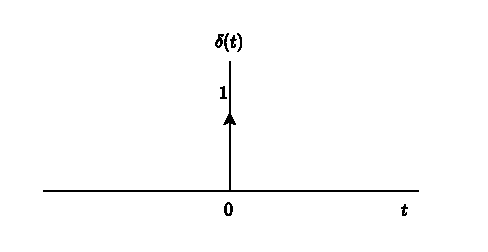
\includegraphics[width=\linewidth]{Fig1.pdf}
    \caption{Continuous-time unit impulse.}
    \label{Fig1}
\end{figure}

As $\Delta\to 0$, $\delta_{\Delta}(t)$ becomes narrower and higher, maintaining its unit area. Its limiting form,
\begin{equation}
    \delta(t) = \lim_{\Delta\to0}\delta_{\Delta}(t),
    \label{1.74}
\end{equation}
can then be thought of as an idealization of the short pulse $\delta_{\Delta}(t)$ as the duration $\Delta$ becomes insignificant. Since $\delta(t)$ has, in effect, no duration but unit area, we adopt the graphical notation for it shown in Figure \ref{Fig1}, where the arrow at $t=0$ indicates that the area of the pulse is concentrated at $t=0$ and the height of the arrow and the "1" next to the arrow are used to represent the \textit{area} of the impulse.

Since the area of the continuous-time unit impulse $\delta(\tau)$ is concentrated at $\tau=0$, we see that the running integral is 0 for $t<0$ and 1 for $t>0$. Also, we note that the relationship in eq.\;(\ref{1.71}) between the continuous-time unit step and impulse can be rewritten in a different form, analogous to the discrete-time form in eq.\;(\ref{1.67}), by changing the variable of integration from $\tau$ to $\sigma=t-\tau$:$$u(t) = \int_{-\infty}^{t}\delta(\tau) d\tau = \int_{\infty}^{0}\delta(t-\sigma)(-d\sigma),$$ or equivalently,
\begin{equation}
    u(t)=\int_0^\infty\delta(t-\sigma) d\sigma.
    \label{1.75}
\end{equation}

As with the discrete-time impulse, the continuous-time impulse has a very important sampling property. In particular, for a number of reasons it will be important to consider the product of an impulse and more well-behaved continuous-time functions $x(t)$. The interpretation of this quantity is most readily developed using the definition of $\delta(t)$ according to eq.\;(\ref{1.74}). Specifically, consider $$x_1(t)=x(t)\delta_{\Delta}(t).$$ By construction, $x_1(t)$ is zero outside the interval $0\le t\le\Delta$. For $\Delta$ sufficiently small so that $x(t)$ is approximately constant over this interval, $$x(t)\delta_{\Delta}(t)\approx x(0)\delta_{\Delta}(t).$$ Since $\delta(t)$ is the limit as $\Delta\to 0$ of $\delta_{\Delta}(t)$, it follows that
\begin{equation}
    x(t)\delta(t)=x(0)\delta(t).
\end{equation}

For systems that respond much more quickly than others, the pulse will have to be of much shorter duration before the details of the pulse shape or its duration no longer matter. Nevertheless, for any physical system, we can always find a pulse that is "short enough." The unit impulse then is an idealization of this concept--the pulse that is short enough for \textit{any} system
\footnotetext[1]{The unit impulse and other related functions (which are often collectively referred to as \textit{singularity functions}) have been thoroughly studied in the field of mathematics under the alternative names of \textit{generalized functions} and the \textit{theory of distributions}.}
.

As a check of our result, we can verify that we can recover $x(t)$ from $\overset{\cdot}{x}(t)$. Specifically, since $x(t)$ and $\overset{\cdot}{x}(t)$ are both zero for $t\le 0$, we need only check that for $t>0$,
\begin{equation}
    x(t)=\int_0^t\overset{\cdot}{x}(\tau)d\tau.
    \label{1.77}
\end{equation}

\section{Continuous-Time and Discrete-Time Systems}

In contexts ranging from signal processing and communications to electromechanical motors, automotive vehicles, and chemical-processing plants, a \textit{system} can be viewed as a process in which input signals are transformed by the system or cause the system to respond in some way, resulting in other signals as outputs.

A \textit{continuous-time system} is a system in which continuous-time input signals are applied and result in continuous-time output signals. Such a system will be represented pictorially as in Figure \ref{Fig2}(a), where $x(t)$ is the input and $y(t)$ is the output. Alternatively, we will often represent the input-output relation of a continuous-time system by the notation
\begin{equation}
    x(t)\to y(t).
    \label{1.78}
\end{equation}

\begin{figure}[htbp]
    \centering
    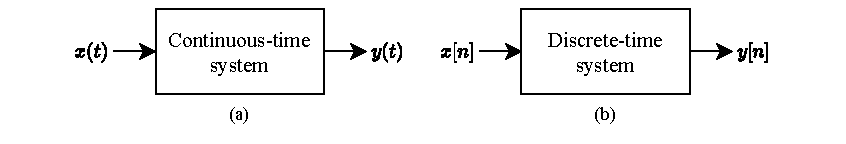
\includegraphics[width=\linewidth]{Fig2.pdf}
    \caption{Continuous-time system}
    \label{Fig2}
\end{figure}

Similarly, a \textit{discrete-time system}--that is, a system that transforms discrete-time inputs into discrete-time outputs--will be depicted as in Figure \ref{Fig2}(b) and will sometimes be represented symbolically as
\begin{equation}
    x[n]\to y[n].
    \label{1.79}
\end{equation}

\subsubsection{Interconnections of Systems}

\begin{figure}[htbp]
    \centering
    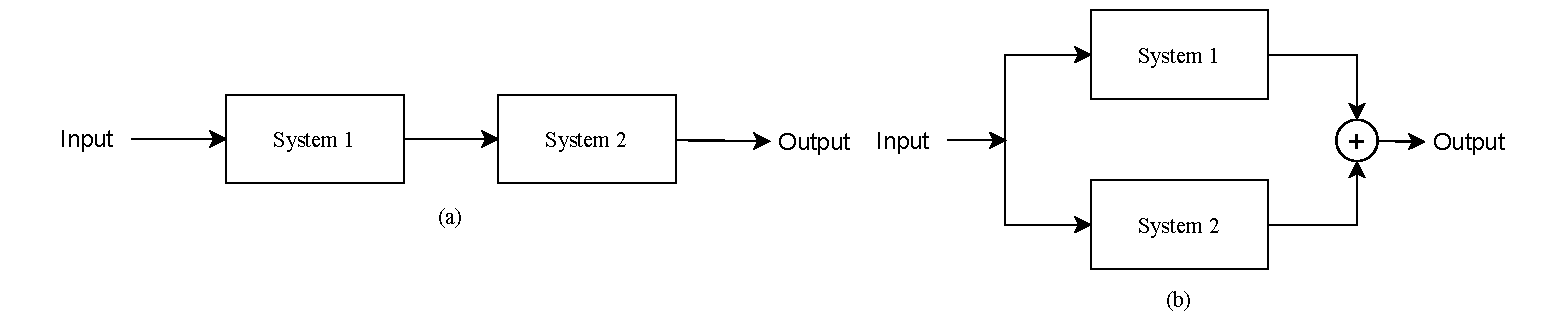
\includegraphics[width=\linewidth]{Fig3.pdf}
    \caption{Interconnection of two systems: (a) series (cascade) interconnection; (b) parallel interconnection.}
    \label{Fig3}
\end{figure}

A \textit{series} or \textit{cascade interconnection} of two systems is illustrated in Figure \ref{Fig3}(a). Diagrams such as this are referred to as \textit{block diagrams}.

A \textit{parallel interconnection} of two systems is illustrated in Figure \ref{Fig3}(b).

Another important type of system interconnection is a \textit{feedback interconncetion}.

\section{Basic System Properties}
\subsection{Systems with and without Memory}
\label{section:1.6.1}

A system is said to be \textit{memoryless} if its output for each value of the independent variable at a given time is dependent on the input at only that same time. A resistor is a memoryless system; with the input $x(t)$ taken as the currnet and with the voltage taken as the output $y(t)$, the input-output relationship of a resistor is
\begin{equation}
    y(t)=Rx(t),
    \label{1.91}
\end{equation}
where $R$ is the resistence. One particularly simple memoryless system is the \textit{identity system}, whose output is identical to its input.

An example of a discrete-time system with memory is an \textit{accumulator} or \textit{summer}
\begin{equation}
    y[n]=\sum\limits_{k=-\infty}^nx[k],
    \label{1.92}
\end{equation}
and a second example is a \textit{delay}
\begin{equation}
    y[n]=x[n-1].
    \label{1.93}
\end{equation}
A capacitor is an example of a continuous-time system with memory, since if the input is taken to be the current and the output is the voltage, then
\begin{equation}
    y(t)=\dfrac1C\int_{-\infty}^tx(\tau)d\tau,
    \label{1.94}
\end{equation}
where $C$ is the capacitance.

Roughly speaking, the concept of memory in a system corresponds to the presence of a mechanism in the system that retains or stores information about input values at times other than the current time. Similarly, the accumulator in eq.\;(\ref{1.92}) must "remember" or store information about past inputs. In particular, the accumulator computes the running sum of all inputs up to the current time, and thus, at each instant of time, the accumulator must add the current input value to the preceding value of the running sum. In other words, the relationship between the input and output of an accumulator can be described as
\begin{equation}
    y[n] = \sum_{k = -\infty}^{n-1}x[k] + x[n],
    \label{1.95}
\end{equation}
or equivalently,
\begin{equation}
    y[n]=y[n-1]+x[n].
    \label{1.96}
\end{equation}

While the concept of memory in a system would typically suggest storing \textit{past} input and output values, our formal definition also leads to our referring to a system as having memory if the current output is dependent on \textit{future} values of the input and output.

\subsection{Invertibility and Inverse Systems}

A system is said to be \textit{invertible} if distinct inputs lead to distinct outputs. If a system is invertible, then an \textit{inverse system} exists that, when cascaded with the original system, yields an output $w[n]$ equal to the input $x[n]$ to the first system.

An example of an invertible system is the accumulator of eq.\;(\ref{1.92}). For this system, the difference between two successive values of the output is precisely the last input value. Therefore, in this case, the inverse system is
\begin{equation}
    w[n]=y[n]-y[n-1].
    \label{1.99}
\end{equation}

For \textit{loseless} coding, the input to the encoder must be exactly recoverable from the output; i.e., the encoder must be invertible.

\subsection{Causality}
\label{section:1.6.3}

A system is \textit{causal} if the output at any time depends on values of the input at only the present and past times. Such a system is often referred to as being \textit{nonanticipative}, as the system output does not anticipate future values of the input.

An example of a noncausal averaging system is
\begin{equation}
    y[n] = \frac{1}{2M+1} \sum_{k = -M}^{+M}x[n-k].
    \label{1.104}
\end{equation}

\subsection{Stablity}
\label{section:1.6.4}

\textit{Stability} is another important system property. Informally, a stable system is one in which small inputs lead to responses that do not diverge. For example, consider the pendulum in Figure \ref{Fig4}(a), in which the input is the applied force $x(t)$ and the output is the angular deviation $y(t)$ from the vertical. In this case, gravity applies a restoring force that tends to return the pendulum to the vertical position, and frictional losses due to drag tend to slow it down. Consequently, if a small force $x(t)$ is applied, the resulting deflection from vertical will also be small. In contrast, for the inverted pendulum in Figure \ref{Fig4}(b), the effect of gravity is to apply a force that tends to \textit{increase} the deviation from vertical.

\begin{figure}[htbp]
    \centering
    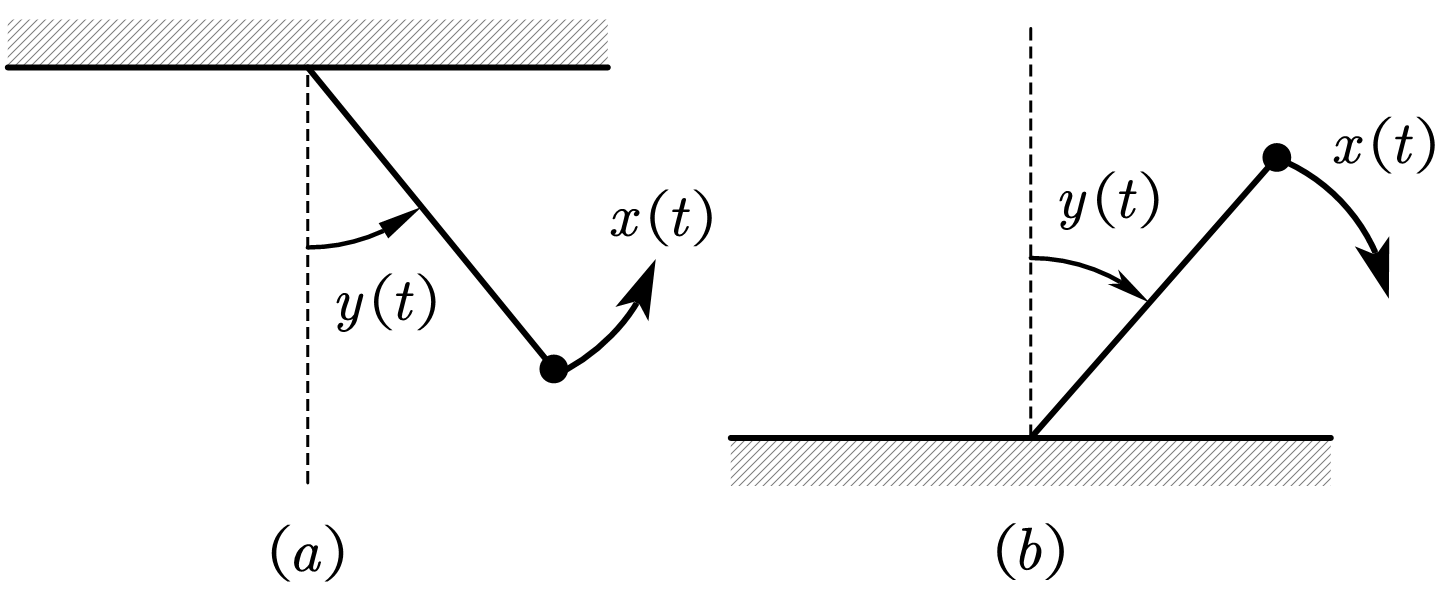
\includegraphics[width=0.35\linewidth]{Fig4.png}
    \caption{(a) A stable pendulum; (b) an unstable inverted pendulum.}
    \label{Fig4}
\end{figure}

As another example, consider the discrete-time system defined by eq.\;(\ref{1.104}), and suppose that the input $x[n]$ is bounded in magnitude by some number, say, $B$, for all values of $n$. Then the largest possible magnitude for $y[n]$ is also $B$, because $y[n]$ is the average of a finite set of values of the input. Therefore, $y[n]$ is bounded and the system is stable. On the other hand, consider the accumulator described by eq.\;(\ref{1.92}). Unlike the system in eq.\;(\ref{1.104}), this system sums \textit{all} of the past values of the input rather than just a finite set of values, and the system is unstable, since the sum can grow continually even if $x[n]$ is bounded.

\subsection{Linearity}

A \textit{linear system}, in continuous time or discrete time, is a system that possesses the important property of superposition: If an input consists of the weighted sum of several signals, then the output is the superposition--that is, the weighted sum--of the responses of the system to each of those signals. More precisely, let $y_1(t)$ be the response of a continuous-time system to an input $x_1(t)$, and let $y_2(t)$ be the output corresponding to the input $x_2(t)$. Then the system is linear if:
\begin{enumerate}
    \item The response to $x_1(t)+x_2(t)$ is $y_1(t)+y_2(t)$.
    \item The response to $ax_1(t)$ is $ay_1(t)$, where $a$ is any complex constant.
\end{enumerate}
The first of these two properties is known as the \textit{additivity} property; the second is known as the \textit{scaling} or \textit{homogeneity} property.

The two properties defining a linear system can be combined into a single statement:
\begin{equation}
    \text{continuous time: }ax_1(t)+bx_2(t)\to ay_1(t)+by_2(t),
    \label{1.121}
\end{equation}
\begin{equation}
    \text{discrete time: }ax_1[n]+bx_2[n]\to ay_1[n]+by_2[n].
    \label{1.122}
\end{equation}
Furthermore, it is straightforward to show from the definition of linearity that if $x_k[n]$, $k=1,2,3,\cdots$, are a set of inputs to a discrete-time linear system with corresponding outputs $y_k[n]$, $k=1,2,3,\cdots$, then the response to a linear combination of these inputs given by
\begin{equation}
    x[n]=\sum_{k}a_{k}x_{k}[n]=a_{1}x_{1}[n]+a_{2}x_{2}[n]+a_{3}x_{3}[n]+\ldots
    \label{1.123}
\end{equation}
is
\begin{equation}
    y[n]=\sum_{k}a_{k}y_{k}[n]=a_{1}y_{1}[n]+a_{2}y_{2}[n]+a_{3}y_{3}[n]+\ldots.
    \label{1.124}
\end{equation}
This very important fact is known as the \textit{superposition property}, which holds for linear systems in both continuous and discrete time.

A direct consequence of the superposition property is that, for linear systems, an input which is zero for all time results in an output which is zero for all time. For example, if $x[n]\to y[n]$, then the homogeneity property tells us that
\begin{equation}
    0=0\cdot x[n]\to0\cdot y[n]=0.
    \label{1.125}
\end{equation}

\chapter{Linear Time-Invariant Systems}
\section{Discrete-Time LTI Systems: The Convolution Sum}
\subsection{The Representation of Discrete-Time Signals in Terms of Impulses}

The key idea in visualizing how the discrete-time unit impulse can be used to construct any discrete-time signal is to think of a discrete-time signal as a sequence of individual impulses. To see how this intuitive picture can be turned into a mathematical representation, consider the signal $x[n]$. For example, $$\left.x[-1]\delta[n+1]=\left\{\begin{array}{ll}{x[-1],}&{n=-1}\\{0,}&{n\neq-1}\\\end{array}\right.\right.,$$$$x[0]\delta[n] = \left\{\begin{array}{ll}{x[0],}&{n = 0}\\{0,}&{n \neq 0}\\\end{array}\right.,$$$$\left.x[1]\delta[n-1]=\left\{\begin{array}{ll}{x[1],}&{n=1}\\{0,}&{n\neq1}\\\end{array}\right.\right..$$ More generally, by including additional shifted, scaled impulses, we can write
\begin{equation}
    \begin{aligned}x[n]=\dots&+ x[-3]\delta[n+3]+ x[-2]\delta[n+2]+ x[-1]\delta[n+1]+ x[0]\delta[n]\\&+ x[1]\delta[n-1]+x[2]\delta[n-2]+x[3]\delta[n-3]+\ldots.\end{aligned}
    \label{2.1}
\end{equation}
For any value of $n$, only one of the terms on the right-hand side of eq.\;(\ref{2.1}) is nonzero, and the scaling associated with that term is precisely $x[n]$. Writing this summation in a more compact form, we have
\begin{equation}
    x[n]=\sum_{k=-\infty}^{+\infty}x[k]\delta[n-k].
    \label{2.2}
\end{equation}

Equation (\ref{2.2}) is called the \textit{sifting property} of the discrete-time unit impulse.

\subsection{The Discrete-Time Unit Impulse Response and the Convolution-Sum Representation of LTI Systems}

The importance of the sifting property of eqs.\;(\ref{2.1}) and (\ref{2.2}) lies in the fact that it represents $x[n]$ as a superposition of scaled versions of a very simple set of elementary functions, namely, shifted unit impulses $\delta[n-k]$, each of which is nonzero (with value 1) at a single point in time specified by the corresponding value of $k$. The response of a linear system to $x[n]$ will be the superposition of the scaled responses of the system to each of these shifted impulses. Moreover, the property of time invariance tells us that the responses of a time-invariant system to the time-shifted unit impulses are simply time-shifted versions of one another. The convolution-sum representation for discrete-time systems that are \textit{both} linear and time invariant results from putting these two basic facts together.

More specifically, consider the response of a linear (but possibly time-varying) system to an arbitrary input $x[n]$. Let $h_k[n]$ denote the response of the linear system to the shifted unit impulse $\delta[n-k]$. Then, from the superposition property for a linear system [eqs.\;(\ref{1.123}) and (\ref{1.124})], the response $y[n]$ of the linear system to the input $x[n]$ in eq.\;(\ref{2.2}) is simply the weighted linear combination of these basic responses. That is, with the input $x[n]$ to a linear system expressed in the form of eq.\;(\ref{2.2}), the output $y[n]$ can be expressed as
\begin{equation}
    y[n] = \sum_{k=-\infty}^{+\infty}x[k]h_{k}[n].
    \label{2.3}
\end{equation}

In general, of course, the responses $h_k[n]$ need not be related to each other for different values of $k$. However, if the linear system is also \textit{time invariant}, then these responses to time-shifted unit impulses are all time-shifted versions of each other. However, if the linear system is also \textit{time invariant}, then these responses to time-shifted unit impulses are all time-shifted versions of each other. Specifically, since $\delta[n-k]$ is time-shifted version of $\delta[n]$, the response $h_k[n]$ is a time-shifted version of $h_[n]$; i.e.,
\begin{equation}
    h_k[n]=h_0[n-k].
    \label{2.4}
\end{equation}
For notational convenience, we will drop the subscript on $h_0[n]$ and define the \textit{unit impulse (sample) response}
\begin{equation}
    h[n]=h_0[n].
    \label{2.5}
\end{equation}
That is, $h[n]$ is the output of the LTI system when $\delta[n]$ is the input. Then for an LTI system, eq.\;(\ref{2.3}) becomes
\begin{equation}
    \boxed{y[n] = \sum_{k = -\infty}^{+\infty}x[k]h[n-k].}
    \label{2.6}
\end{equation}

This result is referred to as the \textit{convolution sum} or \textit{superposition sum}, and the operation on the right-hand side of eq.\;(\ref{2.6}) is known as the \textit{convolution} of the sequences $x[n]$ and $h[n]$. We will represent the operation of convolution symbolically as
\begin{equation}
    y[n]=x[n]*h[n].
    \label{2.7}
\end{equation}

\section{Continuous-Time LTI Systems: The Convolution Integral}
\subsection{The Representation of Continuous-Time Signals in Terms of Impulses}

To develop the continuous-time counterpart of the discrete-time sifting property in eq.\;(\ref{2.2}), we begin by considering a pulse or "staircase" approximation, $\hat{x}(t)$, to a continuous-time signal $x(t)$. If we define
\begin{equation}
    \left.\delta_{\Delta}(t) = \left\{\begin{array}{ll}{\frac{1}{\Delta},}&{0\leq t<\Delta}\\{0,}&{\mathrm{otherwise}}\\\end{array}\right.,\right.
    \label{2.24}
\end{equation}
then, since $\Delta\delta_\Delta(t)$ has unit amplitude, we have the expression
\begin{equation}
    \hat{x}(t) = \sum_{k = -\infty}^{\infty}x(k\Delta)\delta_{\Delta}(t - k\Delta)\Delta.
    \label{2.25}
\end{equation}

As we let $\Delta$ approach 0, the approximation $\hat{x}(t)$ becomes better and better, and in the limit equals $x(t)$. Therefore,
\begin{equation}
    x(t) = \lim_{\Delta\to0}\sum_{k=-\infty}^{+\infty}x(k\Delta)\delta_{\Delta}(t-k\Delta)\Delta.
    \label{2.26}
\end{equation}
Also, as $\Delta\to 0$, the summation in eq.\;(\ref{2.26}) approaches an integral. Moreover, from eq.\;(\ref{1.74}), we know that the limit as $\Delta\to 0$ of $\delta_\Delta(t)$ is the unit impulse function $\delta(t)$. Consequently,
\begin{equation}
    x(t) = \int_{-\infty}^{+\infty}x(\tau)\delta(t-\tau)d\tau.
    \label{2.27}
\end{equation}
As in discrete time, we refer to eq.\;(\ref{2.27}) as the \textit{sifting property} of the continuous-time impulse. We note that, for the specific example of $x(t)=u(t)$, eq.\;(\ref{2.27}) becomes
\begin{equation}
    u(t) = \int_{-\infty}^{+\infty}u(\tau)\delta(t-\tau)d\tau = \int_{0}^{\infty}\delta(t-\tau)d\tau,
    \label{2.28}
\end{equation}
since $u(\tau)=0$ for $\tau<0$ and $u(\tau)=1$ for $\tau>0$.

\subsection{The Continuous-Time Unit Impulse Response and the Convolution Integral Representation of LTI Systems}

As in the discrete-time case, the representation developed in the preceding section provides us with a way in which to view an arbitrary continuous-time signal as the superposition of scaled and shifted pulses. In particular, the approximate representation in eq.\;(\ref{2.25}) represents the signal $\hat{x}(t)$ as a sum of scaled and shifted versions of the basic pulse signal $\delta_\Delta(t)$. Consequently, the response $\hat{y}(t)$ of a linear system to this signal will be the superposition of the responses to the scaled and shifted versions of $\delta_\Delta(t)$. Specifically, let us define $\hat{h}_{k\Delta}(t)$ as the response of an LTI system to the input $\delta_\Delta(t-k\Delta)$. Then, from eq.\;(\ref{2.25}) and the superposition property, for continuous-time linear systems, we see that
\begin{equation}
    \hat{y}(t) = \sum_{k=-\infty}^{+\infty}x(k\Delta)\hat{h}_{k\Delta}(t)\Delta.
    \label{2.29}
\end{equation}
The interpretation of eq.\;(\ref{2.29}) is similar to that for eq.\;(\ref{2.3}) in discrete time.

What remains, then, is to consider what happens as $\Delta$ becomes vanishingly small--i.e., as $\Delta\to 0$. In particular, with $x(t)$ expressed in eq.\;(\ref{2.26}), $\hat{x}(t)$ becomes an increasingly good approximation to $x(t)$, and in fact, the two coincide as $\Delta\to 0$. Consequently, the response to $\hat{x}(t)$, namely, $\hat{y}(t)$ in eq.\;(\ref{2.29}), must converge to $y(t)$, the response to the actual input $x(t)$. Furthermore, as we have said, for $\Delta$ "small enough," the duration of the pulse $\delta_\Delta(t-k\Delta)$ is of no significance, in that, as far as the system is concerned, the response to this pulse is essentially the same as the response to a unit impulse at the same point in time. That is, since the pulse $\delta_\Delta(t-k\Delta)$ corresponds to a shifted unit impulse as $\Delta\to 0$, the response $\hat{h}_{k\Delta}(t)$ to this input pulse becomes the response to an impulse in the limit. Therefore, if we let $h_\tau(t)$ denote the response at time $t$ to a unit impulse $\delta(t-\tau)$ located at time $\tau$, then
\begin{equation}
    y(t) = \lim_{\Delta\to0}\sum_{k=-\infty}^{+\infty}x(k\Delta)\hat{h}_{k\Delta}(t)\Delta.
    \label{2.30}
\end{equation}
As $\delta\to 0$, the summation on the right-hand side becomes an integral. Specifically, as $\Delta\to 0$ the summation approaches the area under $x(\tau)h_\tau(t)$ viewed as a function of $\tau$. Therefore,
\begin{equation}
    y(t) = \int_{-\infty}^{+\infty}x(\tau)h_{\tau}(t)d\tau.
    \label{2.31}
\end{equation}

Equation (\ref{2.31}) represents the general form of the response of a linear system in continuous time. If, in addition to being linear, the system is also time invariant, then $h_\tau(t)=h_0(t-\tau)$; i.e., the response of an LTI system to the unit impulse $\delta(t-\tau)$, which is shifted by $\tau$ seconds from the origin, is a similarly shifted version of the response to the unit impulse function $\delta(t)$. Again, for notational convenience, we will drop the subscript and define the \textit{unit impulse response} $h(t)$ as
\begin{equation}
    h(t)=h_0(t);
\end{equation}
i.e., $h(t)$ is the response to $\delta(t)$. In this case, eq.\;(\ref{2.31}) becomes
\begin{equation}
    \boxed{ y(t) = \int_{-\infty}^{+\infty}x(\tau)h(t-\tau)d\tau.}
    \label{2.33}
\end{equation}

Equation (\ref{2.33}), referred to as the \textit{convolution integral} or the \textit{superposition integral}, is the continuous-time counterpart of the convolution sum of eq.\;(\ref{2.6}) and corresponds to the representation of a continuous-time LTI system in terms of its response to a unit impulse. The convolution of two signals $x(t)$ and $h(t)$ will be represented symbolically as
\begin{equation}
    y(t)=x(t)*h(t).
    \label{2.34}
\end{equation}

\section{Properties of Linear Time-Invariant Systems}

In the preceding two sections, we developed the extremely important representations of continuous-time and discrete-time LTI systems in terms of their unit impulse responses. In discrete time the representation takes the form of the convolution sum, while its continuous-time counterpart is the convolution integral, both of which we repeat here for convenience:
\begin{equation}
    y[n] = \sum_{k=-\infty}^{+\infty}x[k]h[n-k] = x[n]*h[n]
    \label{2.39}
\end{equation}
\begin{equation}
    y(t) = \int_{-\infty}^{+\infty}x(\tau)h(t-\tau)d\tau = x(t)*h(t)
    \label{2.40}
\end{equation}

As we have pointed out, one consequence of these representations is that the characteristics of an LTI system are completely determined by its impulse response. It is important to emphasize that this property holds in general \textit{only} for LTI systems. In particular, the unit impulse response of a nonlinear system does \textit{not} completely characterize the behavior of the system.

\subsection{The Commutative Property}

A basic property of convolution in both continuous and discrete time is that it is a \textit{commutative} operation. That is, in discrete time
\begin{equation}
    x[n]*h[n]= h[n]*x[n] = \sum_{k=-\infty}^{+\infty}h[k]x[n-k],
    \label{2.43}
\end{equation}
and in continuous time
\begin{equation}
    x(t)*h(t)=h(t)*x(t)=\int_{-\infty}^{+\infty}h(\tau)x(t-\tau)d\tau.
    \label{2.44}
\end{equation}
These expressions can be verified in a straightforward manner by means of a substitution of variables in eqs.\;(\ref{2.39}) and (\ref{2.40}). For example, in the discrete-time case, if we let $r=n-k$ or, equivalently, $k=n-r$, eq.\;(\ref{2.39}) becomes
\begin{equation}
    x[n]*h[n]=\sum_{k=-\infty}^{+\infty}x[k]h[n-k]=\sum_{r=-\infty}^{+\infty}x[n-r]h[r]=h[n]*x[n].
    \label{2.45}
\end{equation}

\subsection{The Distributive Property}

Another basic property of convolution is the \textit{distributive} property. Specifically, convolution distributes over addition, so that in discrete time
\begin{equation}
    x[n]*(h_{1}[n]+h_{2}[n])= x[n]*h_{1}[n]+ x[n]*h_{2}[n],
    \label{2.46}
\end{equation}
and in continuous time
\begin{equation}
    x(t)*[h_{1}(t)+h_{2}(t)]=x(t)*h_{1}(t)+x(t)*h_{2}(t).
    \label{2.47}
\end{equation}

\begin{figure}[htbp]
    \centering
    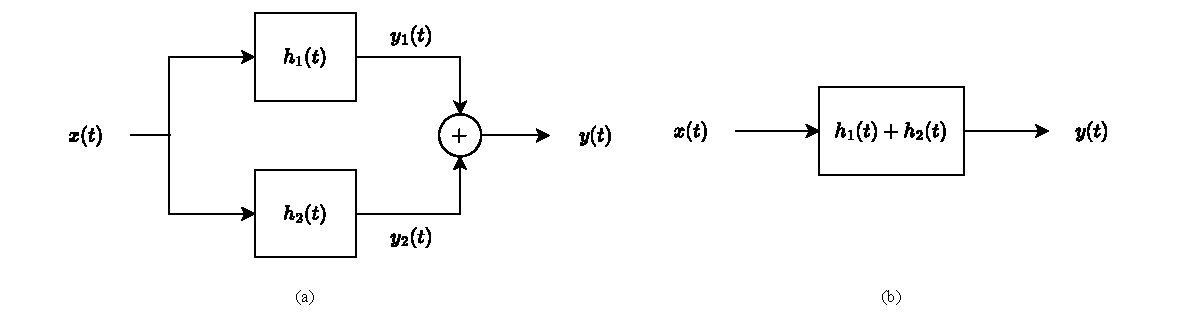
\includegraphics[width=\linewidth]{Fig5.pdf}
    \caption{Interpretation of the distributive property of convolution for a parallel interconnection of LTI systems.}
    \label{Fig5}
\end{figure}

Consider two continuous-time LTI systems in parallel, as indicated in Figure \ref{Fig5}(a).

The two systems, with impulse responses $h_1(t)$ and $h_2(t)$, have identical inputs, and their outputs are added. Since $$y_1(t)=x(t)*h_1(t)$$ and $$y_2(t)=x(t)*h_2(t)$$ the system of Figure \ref{Fig5}(a) has output
\begin{equation}
    y(t) = x(t)*h_1(t)+x(t)*h_2(t),
    \label{2.48}
\end{equation}
corresponding to the right-hand side of eq.\;(\ref{2.47}). The system of Figure \ref{Fig5}(b) has output
\begin{equation}
    y(t) = x(t)*[h_1(t)+h_2(t)],
    \label{2.49}
\end{equation}
corresponding to the left-hand side of eq.\;(\ref{2.47}).

There is an identical interpretation in discrete time, in which each of the signals in Figure \ref{Fig5} is replaced by a discrete-time counterpart (i.e., $x(t)$, $h_1(t)$, $h_2(t)$, $y_1(t)$, $y_2(t)$, and $y(t)$ are replaced by $x[n]$, $h_1[n]$, $h_2[n]$, $y_1[n]$, $y_2[n]$, and $y[n]$, respectively). In summary, then, by virtue of the distributive property of convolution, a parallel combination of LTI systems can be replaced by a single LTI system whose unit impulse response is the sum of the individual unit impulse responses in the parallel combination.

Also, as a consequence of both the commutative and distributive properties, we have
\begin{equation}
    [x_1[n]+x_2[n]]*h[n]=x_1[n]*h[n]+x_2[n]*h[n]
    \label{2.50}
\end{equation}
and
\begin{equation}
    [x_1(t)+x_2(t)]*h(t)=x_1(t)*h(t)+x_2(t)*h(t),
    \label{2.51}
\end{equation}
which simply state that the response of an LTI system to the sum of two inputs must equal the sum of the responses to these signals individually.

\subsection{The Associative Property}

Another important and useful property of convolution is that it is \textit{associative}. That is, in discrete time
\begin{equation}
    x[n]*(h_1[n]*h_2[n])=(x[n]*h_1[n])*h_2[n],
    \label{2.58}
\end{equation}
and in contiunous time
\begin{equation}
    x(t)*[h_1(t)*h_2(t)]\stackrel{\cdot}{=}[x(t)*h_1(t)]*h_2(t).
    \label{2.59}
\end{equation}

As a consequence of the associative property, the expressions
\begin{equation}
    y[n]=x[n]*h_1[n]*h_2[n]
    \label{2.60}
\end{equation}
and
\begin{equation}
    y(t)=x(t)*h_1(t)*h_2(t)
    \label{2.61}
\end{equation}
are unambiguous.

It is important to emphasize that the behavior of LTI systems in cascade--and, in particular, the fact that the overall system response does not depend upon the order of the systems in the cascade--is very special to such systems. In contrast, the order in which nonlinear systems are cascaded cannot be changed, in general, without changing the overall response. Thus, being able to interchange the order of systems in a cascade is a characteristic particular to LTI systems. In fact, we need both linearity \textit{and} time invariance in order for this property to be true in general.

\subsection{LTI Systems with and without Memory}

As specified in Section 1.\ref{section:1.6.1}, a system is memoryless if its output at any time depends only on the value of the input at that same time. From eq.\;(\ref{2.39}), we see that the only way that this can be true for a discrete-time LTI system is if $h[n]=0$ for $n\ne 0$. In this case the impulse response has the form
\begin{equation}
    h[n]=K\delta[n],
    \label{2.62}
\end{equation}
where $K=h[0]$ is a constant, and the convolution sum reduces to the relation
\begin{equation}
    y[n]=Kx[n].
\end{equation}

From eq.\;(\ref{2.40}), we can deduce similar properties for continuous-time LTI systems with and without memory. In particular, a continuous-time LTI system is memoryless if $h(t)=0$ for $t\ne 0$, and such a memoryless LTI system has the form
\begin{equation}
    y(t)=Kx(t)
    \label{2.64}
\end{equation}
for some constant $K$ and has the impulse response
\begin{equation}
    h(t)=K\delta(t).
    \label{2.65}
\end{equation}

\subsection{Invertibility of LTI Systems}

\begin{figure}[htbp]
    \centering
    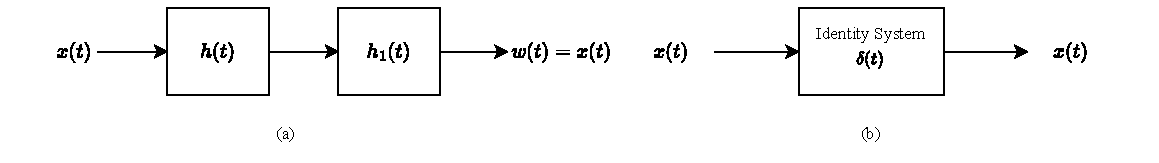
\includegraphics[width=\linewidth]{Fig6.pdf}
    \caption{Concept of an inverse system for continuous-time LTI systems. The system with impulse response $h_1(t)$ is the inverse of the system with impulse response $h(t)$ if $h(t)*h_1(t)=\delta(t)$.}
    \label{Fig6}
\end{figure}

Since the overall impulse response in Figure \ref{Fig6} is $h(t)*h_1(t)$, we have the condition that $h_1(t)$ must satisfy for it to be the impulse response of the inverse system, namely,
\begin{equation}
    h(t)*h_1(t)=\delta(t).
    \label{2.66}
\end{equation}
Similarly, in discrete time, the impulse response $h_1[n]$ of the inverse system for an LTI system with impulse response $h[n]$ must satisfy
\begin{equation}
    h[n]*h_1[n]=\delta[n].
    \label{2.67}
\end{equation}

\subsection{Causality for LTI Systems}

In Section 1.\ref{section:1.6.3}, we introduced the property of causality: The output of a casual system depends only on the present and past values of the input to the system. By using the convolution sum and integral, we can relate this property to a corresponding property of the impulse response of an LTI system. Specifically, in order for a discrete-time LTI system to be casual, $y[n]$ must not depend on $x[k]$ for $k>n$. From eq.\;(\ref{2.39}), we see that for this to be true, all of the coefficients $h[n-k]$ that multiply values of $x[k]$ for $k>n$ must be zero. This then requires that the impulse response of a casual discrete-time LTI system satisfy the condition
\begin{equation}
    h[n]=0\quad\mathrm{for~}n<0.
    \label{2.77}
\end{equation}
According to eq.\;(\ref{2.77}), the impulse response of a casual LTI system must be zero before the impulse occurs, which is consistent with the intuitive concept of causality. More generally, causality for a linear system is equivalent to the condition of \textit{initial rest}; i.e., if the input to a casual system is 0 up to some point in time, then the output must also be 0 up to that time.

For a casual discrete-time LTI system, the condition in eq.\;(\ref{2.77}) implies that the convolution sum representation in eq.\;(\ref{2.39}) becomes
\begin{equation}
    y[n]=\sum_{k=-\infty}^nx[k]h[n-k],
    \label{2.78}
\end{equation}
and the alternative equivalent form, eq.\;(\ref{2.43}), becomes
\begin{equation}
    y[n]=\sum_{k=0}^\infty h[k]x[n-k].
    \label{2.79}
\end{equation}

Similarly, a continuous-time LTI system is causal if
\begin{equation}
    h(t)=0\quad\mathrm{for~}t<0,
    \label{2.80}
\end{equation}
and in this case the convolution integral is given by
\begin{equation}
    y(t)=\int_{-\infty}^{t}x(\tau)h(t-\tau)d\tau=\int_{0}^{\infty}h(\tau)x(t-\tau)d\tau.
    \label{2.81}
\end{equation}

\subsection{Stability for LTI Systems}

Recall from Section 1.\ref{section:1.6.4} that a system is \textit{stable} if every bounded input produces a bounded output. In order to determine conditions under which LTI systems are stable, consider an input $x[n]$ that is bounded in magnitude:
\begin{equation}
    |x[n]|<B\quad\mathrm{for~all~}n.
    \label{2.82}
\end{equation}
Suppose that we apply this input to an LTI system with unit impulse response $h[n]$. Then, using the convolution sum, we obtain an expression for the magnitude of the output:
\begin{equation}
    \left|y[n]\right|=\left|\sum_{k=-\infty}^{+\infty}h[k]x[n-k]\right|.
    \label{2.83}
\end{equation}
Since the magnitude of the sum of a set of numbers is no larger than the sum of the magnitudes of the numbers, it follows from eq.\;(\ref{2.83}) that
\begin{equation}
    |y[n]|\leq\sum_{k=-\infty}^{+\infty}|h[k]||x[n-k]|.
    \label{2.84}
\end{equation}
From eq\;(\ref{2.82}), $|x[n-k]<B|$ for all values of $k$ and $n$. Together with eq.\;(\ref{2.84}), this implies that
\begin{equation}
    |y[n]|\leq B\sum_{k=-\infty}^{+\infty}|h[k]|\quad\text{for all }n.
    \label{2.85}
\end{equation}

From eq.\;(\ref{2.85}), we can conclude that if the impulse response is \textit{absolutely summable}, that is, if
\begin{equation}
    \sum_{k=-\infty}^{+\infty}|h[k]|<\infty,
    \label{2.86}
\end{equation}
then $y[n]$ is bounded in magnitude, and hence, the system is stable.

In continuous time, we obtain an analogous characterization of stability in terms of the impulse responses of an LTI system. Specifically, if $|x(t)|<B$ for all $t$, then, in analogy with eqs.\;(\ref{2.83})-(\ref{2.85}), it follows that $$\begin{aligned}|y(t)|&=\left|\int_{-\infty}^{+\infty}h(\tau)x(t-\tau)d\tau\right|\\&\leq\int_{-\infty}^{+\infty}|h(\tau)||x(t-\tau)|d\tau\\&\leq B\int_{-\infty}^{+\infty}|h(\tau)|d\tau.\end{aligned}$$ Therefore, the system is stable if the impulse response is \textit{absolutely integrable}, i.e., if
\begin{equation}
    \int_{-\infty}^{+\infty}|h(\tau)|d\tau<\infty.
    \label{2.87}
\end{equation}

\subsection{The Unit Step Response of an LTI System}

Up to now, we have seen that the representation of an LTI system in terms of its unit impulse response allows us to obtain very explicit characterizations of system properties. Specifically, since $h[n]$ or $h(t)$ completely determines the behavior of an LTI system, we have been able to relate system properties  to properties of the impulse response.

There is another signal that is also used quite often in describing the behavior of LTI systems: the \textit{unit step response}, $s[n]$ or $s(t)$, corresponding to the output when $x[n]=u[n]$ or $x(t)=u(t)$. From the convolution-sum representation, the step response of a discrete-time LTI system is the convolution of the unit step with the impulse response; that is, $$s[n]=u[n]*h[n].$$ However, by the commutative property of convolution, $s[n]=h[n]*u[n]$, and therefore, $s[n]$ can be viewed as the response to the input $h[n]$ of a discrete-time LTI system with unit impulse response $u[n]$. As we have seen, $u[n]$ is the unit impulse response of the accumulator. Therefore,
\begin{equation}
    s[n]=\sum_{k=-\infty}^nh[k].
    \label{2.91}
\end{equation}
From this equation, it is clear that $h[n]$ can be recovered from $s[n]$ using the relation
\begin{equation}
    h[n]=s[n]-s[n-1].
    \label{2.92}
\end{equation}

Similarly, in continuous time, the step response of an LTI system with impulse response $h(t)$ is given by $s(t)=u(t)*h(t)$, which also equals the response of an integrator [with impulse response $u(t)$] to the input $h(t)$. That is, the unit step response of a continuous-time LTI system is the running integral of its impulse response, or
\begin{equation}
    s(t)=\int_{-\infty}^th(\tau)d\tau,
    \label{2.93}
\end{equation}
and form eq.\;(\ref{2.93}), the unit impulse response is the first derivative of the unit step response, or
\begin{equation}
    h(t)=\frac{ds(t)}{dt}=s^{\prime}(t).
    \label{2.94}
\end{equation}

\section{Causal LTI Systems Described by Differential and Difference Equations}

An extremely important class of continuous-time system is that for which the input and output are related through a \textit{linear constant-coefficient differential equation}.

Correspondingly, an important class of discrete-time systems is that for which the input and output are related through a \textit{linear constant-coefficient difference equation}.

\subsection{Linear Constant-Coefficient Differential Equations}

A very important point about differential equations is that they provide an \textit{implicit} specification of the system.

The homogeneous solution is often referred to as the \textit{natrual response} of the system.

It is important to emphasize that the condition of initial rest does not specify a zero initial condition at a fixed point of time, but rather adjusts this point in time so that the response is zero \textit{until} the input becomes nonzero.

A general $N$th-order linear constant-coefficient differential equation is given by
\begin{equation}
    \sum_{k=0}^Na_k\frac{d^ky(t)}{dt^k}=\sum_{k=0}^Mb_k\frac{d^kx(t)}{dt^k}.
    \label{2.109}
\end{equation}
The order refers to the highest derivative of the output $y(t)$ appearing in the equation. In the case when $N=0$, eq.\;(\ref{2.109}) reduces to
\begin{equation}
    y(t) = \frac{1}{a_0}\sum_{k=0}^Mb_k\frac{d^kx(t)}{dt^k}.
    \label{2.110}
\end{equation}
The solution $y(t)$ consists of two parts--a particular solution to eq.\;(\ref{2.109}) plus a solution to the homogeneous differential equation
\begin{equation}
    \sum_{k=0}^Na_k\frac{d^ky(t)}{dt^k}=0.
    \label{2.111}
\end{equation}
The solutions to this equation are referred to as the \textit{natural responses} of the system.

As in the first-order case, the differential equation (\ref{2.109}) does not completely specify the output in terms of the input, and we need to identify auxiliary conditions to determine completely the input-output relationship for the system. Once again, different choices for these auxiliary conditions result in different input-output relationships, but for the most part, in this book we will use the condition of initial rest when dealing with systems described by differential equations. That is, if $x(t)=0$ for $t\le t_0$, we assume that $y(t)=0$ for $t\le t_0$, and therefore, the response for $t>t_0$ can be calculated from the differential equation (\ref{2.109}) with the initial conditions
\begin{equation}
    y\left(t_0\right)=\frac{dy\left(t_0\right)}{dt}=\ldots=\frac{d^{N-1}y\left(t_0\right)}{dt^{N-1}}=0.
    \label{2.112}
\end{equation}

\subsection{Linear Constant-Coefficient Difference Equations}

The discrete-time counterpart of eq.\;(\ref{2.109}) is the $N$th-order linear constant-coefficient difference equation
\begin{equation}
    \sum_{k=0}^Na_ky[n-k]=\sum_{k=0}^Mb_kx[n-k].
    \label{2.113}
\end{equation}
An equation of this type can be solved in a manner exactly analogous to that for differential equations. Specifically, the solution $y[n]$ can be written as the sum of a particular solution to eq.\;(\ref{2.113}) and a solution to the homogeneous equation
\begin{equation}
    \sum_{k=0}^Na_ky[n-k]=0.
    \label{2.114}
\end{equation}

Although all of these properties can be developed following an approach that directly parallels our discussion for differential equations, the discrete-time case offers an alternative path. This stems from the observation that eq.\;(\ref{2.113}) can be rearranged in the form
\begin{equation}
    y[n] = \frac{1}{a_0}\left\{\sum_{k=0}^Mb_kx[n-k]-\sum_{k=1}^Na_ky[n-k]\right\}.
    \label{2.115}
\end{equation}

An equation of the form of eq.\;(\ref{2.113}) or eq.\;(\ref{2.115}) is called a \textit{recursive equation}, since it specifies a recursive procedure for determining the output in terms of the input and previous outputs. In the special case when $N=0$, eq.\;(\ref{2.115}) reduces to
\begin{equation}
    y[n] = \sum_{k=0}^M\biggl(\frac{b_k}{a_0}\biggr)x[n-k].
    \label{2.116}
\end{equation}
Here, $y[n]$ is an explicit function of the present and previous values of the input. For this reason, eq.\;(\ref{2.116}) is often called a \textit{nonrecursive equation}, since we do not recursively use previously computed values of the output to compute the present value of the output. Therefore, just as in the case of the system given in eq.\;(\ref{2.110}), we do not need auxiliary conditions in order to determine $y[n]$. Furthermore, eq.\;(\ref{2.116}) describes an LTI system, and by direct computation, the impulse response of this system is found to be
\begin{equation}
    \left.h[n]=\left\{\begin{array}{ll}\frac{b_n}{a_0},&0\leq n\leq M\\0,&\text{otherwise}\end{array}\right.\right..
    \label{2.117}
\end{equation}
Note that the impulse response for it has finite duration; that is, it is nonzero only over a finite time interval. Because of this property, the system specified by eq.\;(\ref{2.116}) is often called a \textit{finite impulse response (FIR) system}.

In fact, if $N\ge 1$ in eq.\;(\ref{2.113}), so that the difference equation is recursive, it is usually the case that the LTI system corresponding to this equation together with the condition of initial rest will have an impulse response of infinite duration. Such systems are commonly referred to as \textit{infinite impulse response (IIR) systems}.

\subsection{Block Diagram Representations of First-Order Systems Described by Differential and Difference Equations}

We begin with the discrete-time case and, in particular, the causal system described by the first-order difference equation
\begin{equation}
    y[n]+ay[n-1]=bx[n].
    \label{2.126}
\end{equation}
To develop a block diagram representation of this system, note that the evaluation of eq.\;(\ref{2.126}) requires three basic operations: addition, multiplication by a coefficient, and delay (to capture the relationship between $y[n]$ and $y[n-1]$). Thus, let us define three basic network elements, as indicated in Figure \ref{Fig7}. To see how these basic elements can be used to represent the causal system described by eq.\;(\ref{2.126}), we rewrite this equation in the form that directly suggests a recursive algorithm for computing successive values of the output $y[n]$:
\begin{equation}
    y[n]=-ay[n-1]+bx[n].
    \label{2.127}
\end{equation}

\begin{figure}[htbp]
    \centering
    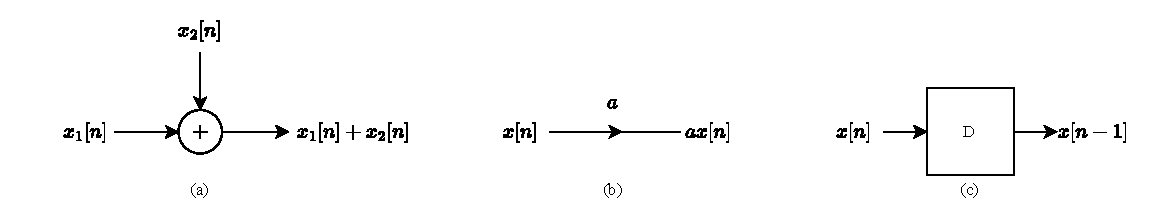
\includegraphics[width=\linewidth]{Fig7.pdf}
    \caption{Basic elements for the block diagram representation of the causal system described by eq.\;(\ref{2.126}): (a) an adder; (b) multiplication by a coefficient; (c) a unit delay.}
    \label{Fig7}
\end{figure}

Consider next the causal continuous-time system described by a first-order differential equation:
\begin{equation}
    \dfrac{dy(t)}{dt}+ay(t)=bx(t).
    \label{2.128}
\end{equation}
As a first attempt at defining a block diagram representation for this system, let us rewrite it as
\begin{equation}
    y(t)=-\dfrac{1}{a}\dfrac{dy(t)}{dt}+\dfrac{b}{a}x(t).
    \label{2.129}
\end{equation}

An alternative implementation that is much more widely used can be obtained by first rewriting eq.\;(\ref{2.128}) as
\begin{equation}
    \dfrac{dy(t)}{dt}=bx(t)-ay(t)
    \label{2.130}
\end{equation}
and then integrating from $-\infty$ to $t$. Specifically, if we assume that in the system describd by eq.\;(\ref{2.130}) the value of $y(-\infty)$ is zero, then the integral of $dy(t)/dt$ from $-\infty$ to $t$ is precisely $y(t)$. Consequently, we obtain the equation
\begin{equation}
    y(t) = \int_{-\infty}^t\left[bx(\tau)-ay(\tau)\right] d\tau.
    \label{2.131}
\end{equation}
In this form, our system can be implemented using the adder and coefficient multiplier, together with an \textit{integrator}.

Note that in the continuous-time case it is the integrator that represents the memory storage element of the system. This is perhaps more readily seen if we consider integrating eq.\;(\ref{2.130}) from a finite point in time $t_0$, resulting in the expression
\begin{equation}
    y(t) = y(t_0)+\int_{t_0}^t\left[bx(\tau)-ay(\tau)\right]d\tau.
    \label{2.132}
\end{equation}

\section{Singularity Functions}
\subsection{The Unit Impulse as an Idealized Short Pulse}

From the sifting property, eq.\;(\ref{2.27}), the unit impulse $\delta(t)$ is the impulse response of the identity system. That is,
\begin{equation}
    x(t)=x(t)*\delta(t)
    \label{2.133}
\end{equation}
for any signal $x(t)$. Therefore, if we take $x(t)=\delta(t)$, we have
\begin{equation}
    \delta(t)=\delta(t)*\delta(t).
    \label{2.134}
\end{equation}
Equation (\ref{2.134}) is a basic property of the unit impulse, and it also has a significant implication for our interpretation of the unit impulse as an idealized pulse. Specifically, let $\delta_\Delta(t)$ correspond to the rectangular pulse, and let
\begin{equation}
    r_\Delta(t)=\delta_\Delta(t)*\delta_\Delta(t).
    \label{2.135}
\end{equation}

\subsection{Defining the Unit Impulse through Convolution}

While usually a function or signal is defined by what it is at each value of the independent variable, the primary importance of the unit impulse is not what it \textit{is} at each value of $t$, but rather what it \textit{does} under convolution. Thus, from the point of view of linear systems analysis, we may alternatively \textit{define} the unit impulse as that signal which, when applied to an LTI system, yields the impulse response. That is, we define $\delta(t)$ as the signal for which
\begin{equation}
    x(t)=x(t)*\delta(t)
    \label{2.138}
\end{equation}
for any $x(t)$.

All the properties of the unit impulse that we need can be obtained from the \textit{operational definition} given by eq.\;(\ref{2.138}).

It is sometimes useful to use another completely equivalent operational definition of $\delta(t)$. To obtain this alternative form, consider taking an arbitrary signal $g(t)$, reversing it in time to obtain $g(-t)$, and then convolving this with $\delta(t)$. Using eq.\;(\ref{2.138}), we obtain $$g(-t)= g(-t)*\delta(t)=\int_{-\infty}^{+\infty}g(\tau-t) \delta(\tau) d\tau,$$ which, for $t=0$, yields
\begin{equation}
    g(0)=\int_{-\infty}^{+\infty}g(\tau)\delta(\tau)d\tau.
    \label{2.139}
\end{equation}

Since we will be concerned principally with LTI systems, and thus with convolution, the characterization of $\delta(t)$ given in eq.\;(\ref{2.138}) will be the one to which we will refer most often. However, eq.\;(\ref{2.139}) is useful in determining some of other properties of the unit impulse. For example, consider the signal $f(t)\delta(t)$, where $f(t)$ is another signal. Then, from eq.\;(\ref{2.139}),
\begin{equation}
    \int_{-\infty}^{+\infty}g(\tau)f(\tau)\delta(\tau)d\tau=g(0)f(0).
    \label{2.140}
\end{equation}
On the other hand, if we consider the signal $f(0)\delta(t)$, we see that
\begin{equation}
    \int_{-\infty}^{+\infty}g(\tau)f(0) \delta(\tau) d\tau= g(0)f(0).
    \label{2.141}
\end{equation}
Comparing eqs.\;(\ref{2.140}) and (\ref{2.141}), we find that the two signals $f(t)\delta(t)$ and $f(0)\delta(t)$ behave identically when they are multiplied by any signal $g(t)$ and then integrated from $-\infty$ to $+\infty$. Consequently, using this form of the operational definition of signals, we conclude that
\begin{equation}
    f(t)\delta(t)=f(0)\delta(t),
    \label{2.142}
\end{equation}
which is property that we derived by alternative means in Section 1.\ref{section:1.4.2}.

\subsection{Unit Doublets and Other Singularity Functions}

The unit impulse is one of a class of signals known as \textit{singularity functions}, each of which can be defined operationally in terms of its behavior under convolution. Consider the LTI system for which the output is the derivative of the input, i.e.,
\begin{equation}
    y(t)=\dfrac{dx(t)}{dt}
    \label{2.143}
\end{equation}
The unit impulse response of this system is the derivative of the unit impulse, which is called the \textit{unit doublet} $u_1(t)$. From the convolution representation for LTI systems, we have
\begin{equation}
    \frac{dx(t)}{dt}=x(t)*u_1(t)
    \label{2.144}
\end{equation}
for any signal $x(t)$. Just as eq.\;(\ref{2.138}) serves as the operational definition of $\delta(t)$, we will take eq.\;(\ref{2.144}) as the operational definition of $u_1(t)$. Similarly, we can define $u_2(t)$, the second derivative of $\delta(t)$, as the impulse response of an LTI system that takes the second derivative of the input, i.e.,
\begin{equation}
    \frac{d^2x(t)}{dt^2}=x(t)*u_2(t).
    \label{2.145}
\end{equation}
From eq.\;(\ref{2.144}), we see that
\begin{equation}
    \frac{d^2x(t)}{dt^2}=\frac d{dt}\left(\frac{dx(t)}{dt}\right)=x(t)*u_1(t)*u_1(t),
    \label{2.146}
\end{equation}
and therefore,
\begin{equation}
    u_2(t)=u_1(t)*u_1(t).
    \label{2.147}
\end{equation}
In general, $u_k(t)$, $k>0$, is the $k$th derivative of $\delta(t)$ and thus is the impulse response of a system that takes the $k$th derivative of the input. Since this system can be obtained as the cascade of $k$ differentiators, we have
\begin{equation}
    u_k(t)=\underbrace{u_1(t)*\cdots*u_1(t)}_{k\mathrm{~times}}.
    \label{2.148}
\end{equation}

As with the unit impulse, each of these singularity functions has properties that can be derived from its operational definition. For example, if we consider the constant signal $x(t)=1$, we find that $$\begin{aligned}0=\frac{dx(t)}{dt}&= x(t)*u_{1}(t)=\int_{-\infty}^{+\infty}u_{1}(\tau)x(t-\tau) d\tau\\&=\int_{-\infty}^{+\infty}u_{1}(\tau) d\tau,\end{aligned}$$ so that the unit doublet has zero area. Moreover, if we convolve the signal $g(-t)$ with $u_1(t)$, we obtain $$\int_{-\infty}^{+\infty}g(\tau-t)u_1(\tau) d\tau= g(-t)*u_1(t) = \frac{dg(-t)}{dt} = -g^{\prime}(-t),$$ which, for $t=0$, yields
\begin{equation}
    -g^{\prime}(0) = \int_{-\infty}^{+\infty}g(\tau)u_1(\tau) d\tau.
    \label{2.149}
\end{equation}

As with the unit impulse, each of these singularity functions can be informally related to short pulses. For instance, consider the short pulse $\delta_\Delta(t)$. This pulse behaves like an impulse as $\Delta\to 0$. Consequently, we would expect its derivative to behave like a doublet as $\Delta\to 0$. $d\delta_\Delta/dt$ consists of a unit impulse at $t=0$ with area $+1/\Delta$, followed by a unit impulse of area $-1/\Delta$ at $t=\Delta$, i.e.,
\begin{equation}
    \frac{d\delta_\Delta(t)}{dt}=\frac1\Delta[\delta(t)-\delta(t-\Delta)].
    \label{2.150}
\end{equation}
Consequently, using the fact that $x(t)*\delta(t-t_0)=x(t-t_0)$, we find that
\begin{equation}
    x(t)*\frac{d\delta_\Delta(t)}{dt}=\frac{x(t)-x(t-\Delta)}\Delta\cong\frac{dx(t)}{dt},
    \label{2.151}
\end{equation}
where the approximation becomes increasingly accurate as $\Delta\to 0$.

The unit step is the impulse response of an integrator: $$y(t)=\int_{-\infty}^tx(\tau) d\tau.$$ Therefore,
\begin{equation}
    u(t)=\int_{-\infty}^t\delta(\tau) d\tau,
    \label{2.152}
\end{equation}
and we also have the following operational definition of $u(t)$:
\begin{equation}
    x(t)*u(t)=\int_{-\infty}^tx(\tau) d\tau.
    \label{2.153}
\end{equation}

Similarly, we can define the system that consists of a cascade of two integrators. Its impulse response is denoted by $u_{-2}(t)$, which is simply the convolution of $u(t)$, the impulse response of one integrator, with itself:
\begin{equation}
    u_{-2}(t) = u(t)*u(t) = \int_{-\infty}^{t}u(\tau) d\tau.
    \label{2.154}
\end{equation}
Since $u(t)$ equals 0 for $t<0$ and equals 1 for $t>0$, it follows that
\begin{equation}
    u_{-2}(t)=tu(t).
    \label{2.155}
\end{equation}
This signal, which is referred to as the \textit{unit ramp function}. Also, we can obtain an operational definition for the behavior of $u_{-2}(t)$ under convolution from eqs.\;(\ref{2.153}) and (\ref{2.154}):
\begin{equation}
    \begin{aligned}x(t)*u_{-2}(t)&= x(t)*u(t)*u(t)\\&=\left(\int_{-\infty}^{t}x(\sigma) d\sigma\right)*u(t)\\&=\int_{-\infty}^{t}\left(\int_{-\infty}^{\tau}x(\sigma) d\sigma\right)d\tau.\end{aligned}
    \label{2.156}
\end{equation}

In an analogous fashion, we can define higher order integrals of $\delta(t)$ as the impulse responses of cascades of integrators:
\begin{equation}
    u_{-k}(t)=\underbrace{u(t)*\cdots*u(t)}_{k\mathrm{~times}}=\int_{-\infty}^{t}u_{-(k-1)}(\tau) d\tau.
    \label{2.157}
\end{equation}
The convolution of $x(t)$ with $u_{-3}(t)$, $u_{-4}(t)$, $\ldots$ generate correspondingly higher order integrals of $x(t)$. Also, note that the integrals in eq.\;(\ref{2.157}) can be evaluated directly, as we done in eq.\;(\ref{2.155}), to obtain
\begin{equation}
    u_{-k}(t)=\frac{t^{k-1}}{(k-1)!}u(t).
    \label{2.158}
\end{equation}

At times it will be worthwhile to use an alternative notation for $\delta(t)$ and $u(t)$, namely,
\begin{equation}
    \delta(t)=u_0(t),
    \label{2.159}
\end{equation}
\begin{equation}
    u(t)=u_{-1}(t).
    \label{2.160}
\end{equation}
With this notation, $u_k(t)$ for $k>0$ denotes the impulse response of a cascade of $k$ differentiators, $u_0(t)$ is the impulse response of the identity system, and, for $k<0$, $u_k(t)$ is the impulse response of a cascade of $|k|$ integrators. Furthermore, since a differentiator is the inverse system of an integrator, $$u(t)*u_1(t)=\delta(t),$$ or, in our alternative notation,
\begin{equation}
    u_{-1}(t)*u_1(t)=u_0(t).
    \label{2.161}
\end{equation}
More generally, from eqs.\;(\ref{2.148}), (\ref{2.157}), and (\ref{2.161}), we see that for any integers $k$ and $r$,
\begin{equation}
    u_k(t)*u_r(t)=u_{k+r}(t).
    \label{2.162}
\end{equation}
\footnotetext[1]{As mentioned in Chapter 1, singularity functions have been heavily studied in the field of mathematics under the alternative names of \textit{generalized functions} and \textit{distribution theory}.}

\chapter{Fourier Series Representation of Periodic Signals}
\section{A Historical Perspective}

By 1807, Fourier had completed a work, Fourier had found series of harmonically related sinusoids to be useful in representing the temperature distribution through a body. In addition, he claimed that "any" period signal could be represented by such a series. While his treatment of this topic was significant, many of the basic ideas behind it had been discovered by others. Also, Fourier's mathematical arguments were still imprecise, and it remained for P.L. Dirichlet in 1829 to provide precise conditions under which a periodic signal could be represented by a Fourier series. Thus, Fourier did not actually contribute to the mathematical theory of Fourier series. However, he did have the clear insight to see the potential for this series representation, and it was to a great extent his work and his claims that spurred much of the subsequent work on Fourier series. In addition, Fourier took this type of representation one very large step farther than any of his predecessors: He obtained a representation for \textit{aperiodic} signals--not as weighted \textit{sums} of harmonically related sinusoids--but as weighted \textit{integrals} of sinusoids that are \textit{not} all harmonically related.

Alternating-current sources generate sinusoidal voltages and currents, and the tools of Fourier analysis enable us to analyze the response of an LTI system to such sinusoidal inputs. Also, waves in the ocean consist of the linear combination of sinusoidal waves with different spatial periods or \textit{wavelengths}.

\section{The Response of LTI Systems to Complex Exponentials}
\label{section:3.2}

The importance of complex exponentials in the study of LTI systems stems from the fact that the response of an LTI system to a complex exponential input is the same complex exponential with only a change in amplitude; that is,
\begin{equation}
    \text{continuous time: }e^{st}\longrightarrow H(s)e^{st},
    \label{3.1}
\end{equation}
\begin{equation}
    \text{discrete time: }z^n\longrightarrow H(z)z^n,
    \label{3.2}
\end{equation}
where the complex amplitude factor $H(s)$ or $H(z)$ will in general be a function of the complex variable $s$ or $z$. A signal for which the system output is a (possibly complex) constant times the input is referred to as an \textit{eigenfunction} of the system, and the amplitude factor is referred to as the system's \textit{eigenvalue}.

To show that complex exponentials are indeed eigenfunctions of LTI systems, let us consider a continuous-time LTI system with impulse response $h(t)$. For an input $x(t)$, we can determine the output through the use of the convolution integral, so that with $x(t)=e^{st}$
\begin{equation}
    \begin{aligned}y(t)&=\int_{-\infty}^{+\infty}h(\tau)x(t-\tau) d\tau\\&=\int_{-\infty}^{+\infty}h(\tau)e^{s(t-\tau)} d\tau.\end{aligned}
    \label{3.3}
\end{equation}
Expressing $e^{s(t-\tau)}$ as $e^{st}e^{-s\tau}$, and noting that $e^{st}$ can be moved outside the integral, we see that eq.\;(\ref{3.3}) becomes
\begin{equation}
    y(t) = e^{st}\int_{-\infty}^{+\infty}h(\tau)e^{-s\tau} d\tau.
    \label{3.4}
\end{equation}
Assuming that the integral on the right-hand side of eq.\;(\ref{3.4}) converges, the response to $e^{st}$ is of the form
\begin{equation}
    y(t)=H(s)e^{st},
    \label{3.5}
\end{equation}
where $H(s)$ is a complex constant whose value depends on $s$ and which is related to the system impulse response by
\begin{equation}
    H(s)=\int_{-\infty}^{+\infty}h(\tau)e^{-s\tau} d\tau.
    \label{3.6}
\end{equation}

In an exactly parallel manner, we can show that complex exponential sequences are eigenfunctions of discrete-time LTI systems. That is, suppose that an LTI system with impulse response $h[n]$ has as its input the sequence
\begin{equation}
    x[n]=z^n,
    \label{3.7}
\end{equation}
where $z$ is a complex number. Then the output of the system can be determined from the convolution sum as
\begin{equation}
    \begin{aligned}y[n]&=\sum_{k=-\infty}^{+\infty}h[k]x[n-k]\\&=\sum_{k=-\infty}^{+\infty}h[k]z^{n-k}=z^{n}\sum_{k=-\infty}^{+\infty}h[k]z^{-k}.\end{aligned}
    \label{3.8}
\end{equation}
From this expression, we see that if the input $x[n]$ is the complex exponential given by eq.\;(\ref{3.7}), then, assuming that the summation on the right-hand side of eq.\;(\ref{3.8}) converges, the output is the same complex exponential multiplied by a constant that depends on the value of $z$. That is,
\begin{equation}
    y[n]=H(z)z^n,
    \label{3.9}
\end{equation}
where
\begin{equation}
    H(z)=\sum_{k=-\infty}^{+\infty}h[k]z^{-k}.
    \label{3.10}
\end{equation}

Let $x(t)$ correspond to a linear combination of three complex exponentials; that is,
\begin{equation}
    x(t)=a_1e^{s_1t}+a_2e^{s_2t}+a_3e^{s_3t}.
    \label{3.11}
\end{equation}
From the eigenfunction property, the response to each separately is $$a_1e^{s_1t}\longrightarrow a_1H(s_1)e^{s_1t},$$$$a_2e^{s_2t}\longrightarrow a_2H(s_2)e^{s_2t},$$$$a_3e^{s_3t}\longrightarrow a_3H(s_3)e^{s_3t},$$ and from the superposition property the response to the sum is the sum of the responses, so that
\begin{equation}
    y(t)=a_1H(s_1)e^{s_1t}+a_2H(s_2)e^{s_2t}+a_3H(s_3)e^{s_3t}.
    \label{3.12}
\end{equation}
More generally, in continuous time, eq.\;(\ref{3.5}), together with the superposition property, implies that the representation of signals as a linear combination of complex exponentials leads to a convenient expression for the response of an LTI system. Specifically, if the input to a continuous-time LTI system is represented as a linear combination of complex exponentials, that is, if
\begin{equation}
    x(t)=\sum_ka_ke^{s_kt},
    \label{3.13}
\end{equation}
then the output will be
\begin{equation}
    y(t)=\sum_ka_kH(s_k)e^{s_kt}.
    \label{3.14}
\end{equation}
In an exactly analogous manner, if the input to a discrete-time LTI system is represented as a linear combination of complex exponentials, that is, if
\begin{equation}
    x[n]=\sum_ka_kz_k^n,
    \label{3.15}
\end{equation}
then the output will be
\begin{equation}
    y[n]=\sum_ka_kH(z_k)z_k^n.
    \label{3.16}
\end{equation}

\section{Fourier Series Representation of Continuous-Time Periodic Signals}
\label{section:3.3}

\subsection{Linear Combinations of Harmonically Related Complex Exponentials}

As defined in Chapter \ref{chapter:1}, a signal is periodic if, for some positive value of $T$,
\begin{equation}
    x(t) = x(t + T)\quad\text{for all }t.
    \label{3.21}
\end{equation}

In Chapter \ref{chapter:1} we also introduced two basic periodic signals, the sinusoidal signal
\begin{equation}
    x(t)=\cos\omega_0t
    \label{3.22}
\end{equation}
and the periodic complex exponential
\begin{equation}
    x(t)=e^{j\omega_0t}.
    \label{3.23}
\end{equation}
Associated with the signal in eq.\;(\ref{3.23}) is the set of \textit{harmonically related} complex exponentials
\begin{equation}
    \phi_k(t) = e^{jk\omega_0t} = e^{jk(2\pi/T)t},\quad k = 0,\pm1,\pm2,\ldots.
    \label{3.24}
\end{equation}
Each of these signals has a fundamental frequency that is a multiple of $\omega_0$, and therefore, each is periodic with period $T$ (although for $|k|\ge 2$, the fundamental period of $\phi_k(t)$ is a fraction of $T$). Thus, a linear combination of harmonically related complex exponentials of the form
\begin{equation}
    x(t) = \sum_{k=-\infty}^{+\infty}a_ke^{jk\omega_0t} = \sum_{k=-\infty}^{+\infty}a_ke^{jk(2\pi/T)t}
    \label{3.25}
\end{equation}
is also periodic with period $T$. The terms for $k=+1$ and $k=-1$ both have fundamental frequency equal to $\omega_0$ and are collectively referred to as the \textit{fundamental components} or the \textit{first harmonic components}. The two terms for $k=+2$ and $k=-2$ are periodic with half the period (or, equivalently, twice the frequency) of the fundamental components and are referred to as the \textit{second harmonic components}.

The representation of a periodic signal in the form of eq.\;(\ref{3.25}) is referred to as the \textit{Fourier series} representation.

Specifically, suppose that $x(t)$ is real and can be represented in the form of eq.\;(\ref{3.25}). Then, since $x^{*}(t)=x(t)$, we obtain $$x(t) = \sum_{k=-\infty}^{+\infty}a_{k}^{*}e^{-jk\omega_{0}t}.$$

Replacing $k$ by $-k$ in the summation, we have $$x(t) = \sum_{k=-\infty}^{+\infty}a_{-k}^{*}e^{jk\omega_{0}t},$$ which, by comparison with eq.\;(\ref{3.25}), requires that $a_k=a_{-k}^*$, or equivalently, that
\begin{equation}
    a_k^*=a_{-k}.
    \label{3.29}
\end{equation}

To derive the alternative forms of the Fourier series, we first rearrange the summation in eq.\;(\ref{3.25}) as $$    x(t) = a_{0}+\sum_{k=1}^{\infty}[a_{k}e^{jk\omega_{0}t} + a_{-k}e^{-jk\omega_{0}t}].$$ Substituting $a_k^*$ for $a_{-k}$ from eq.\;(\ref{3.29}), we obtain $$x(t)=a_0+\sum_{k=1}^\infty[a_ke^{jk\omega_0t}+a_k^*e^{-jk\omega_0t}].$$ Since the two terms inside the summation are complex conjugates of each other, this can be expressed as
\begin{equation}
    x(t)=a_0+\sum_{k=1}^\infty2\Re e\{a_ke^{jk\omega_0t}\}.
    \label{3.30}
\end{equation}
If $a_k$ if expressed in polar form as $$a_k=A_ke^{j\theta_k},$$ then eq.\;(\ref{3.30}) becomes $$x(t) = a_0 + \sum_{k=1}^{\infty}2\Re e\{A_ke^{j(k\omega_0t+\theta_k)}\}.$$ That is,
\begin{equation}
    x(t)=a_0+2\sum_{k=1}^\infty A_k\cos(k\omega_0t+\theta_k).
    \label{3.31}
\end{equation}
Equation\;(\ref{3.31}) is one commonly encountered form for the Fourier series of real periodic signals in continuous time. Another form is obtained by writing $a_k$ in rectangular form as $$a_k=B_k+jC_k,$$ where $B_k$ and $C_k$ are both real. With this expression for $a_k$, eq.\;(\ref{3.30}) takes the form
\begin{equation}
    x(t)=a_0+2\sum_{k=1}^\infty[B_k\cos k\omega_0t-C_k\sin k\omega_0t].
    \label{3.32}
\end{equation}

\subsection{Determination of the Fourier Series Representation of a Continuous-time Periodic Signal}

Multiplying both sides of eq.\;(\ref{3.25}) by $e^{-jn\omega_0t}$, we obtain
\begin{equation}
    x(t)e^{-jn\omega_0t}=\sum_{k=-\infty}^{+\infty}a_ke^{jk\omega_0t}e^{-jn\omega_0t}.
    \label{3.33}
\end{equation}
Integrating both sides from 0 to $T=2\pi/\omega_0$, we have $$\int_0^Tx(t)e^{-jn\omega_0t} dt = \int_0^T\sum_{k=-\infty}^{+\infty}a_ke^{jk\omega_0t}e^{-jn\omega_0t} dt.$$ Interchanging the order of integration and summation yields
\begin{equation}
    \int_0^Tx(t)e^{-jn\omega_0t} dt = \sum_{k=-\infty}^{+\infty}a_k\bigg[\int_0^Te^{j(k-n)\omega_0t} dt\bigg].
    \label{3.34}
\end{equation}
Rewriting this integral using Euler's formula, we obtain
\begin{equation}
    \int_0^Te^{j(k-n)\omega_0t} dt = \int_0^T\cos(k-n)\omega_0t dt + j\int_0^T\sin(k-n)\omega_0t dt.
    \label{3.35}
\end{equation}
Since the integral may be viewed as measuring the total area under the functions over the interval, we see that for $k\ne n$, both of the integrals on the right-hand side of eq.\;(\ref{3.35}) are zero. For $k=n$, the integrand on the left-hand side of eq.\;(\ref{3.35}) equals 1, and thus, the integral equals $T$. In sum, we then have $$\left.\int_0^Te^{j(k-n)\omega_0t} dt=\left\{\begin{array}{ll}T,&k=n\\0,&k\neq n\end{array}\right.\right.,$$ and consequently, the right-hand side of eq.\;(\ref{3.34}) reduces to $Ta_n$. Therefore,
\begin{equation}
    a_n=\frac{1}{T}\int_0^Tx(t)e^{-jn\omega_0t} dt,
    \label{3.36}
\end{equation}
which provides the equation for determining the coefficients. Futhermore, note that in evaluating eq.\;(\ref{3.35}), the only fact that we used concerning the interval of integration was that we were integrating over an interval of length $T$, which is an integral number of periods of $\cos(k-n)\omega_0t$ and $\sin(k-n)\omega_0t$. Therefore, we will obtain the same result if we integrate over any interval of length $T$. That is, if we denote integration over \textit{any} interval of length $T$ by $\int_T$, we have $$\left.\int_Te^{j(k-n)\omega_0t} dt=\left\{\begin{array}{ll}T,&k=n\\0,&k\neq n\end{array}\right.\right.,$$ and consequently,
\begin{equation}
    a_n = \frac1T\int_Tx(t)e^{-jn\omega_0t} dt.
    \label{3.37}
\end{equation}

To summarize, if $x(t)$ has a Fourier series representation [i.e., if it can be expressed as a linear combination of harmonically related complex exponentials in the form of eq.\;(\ref{3.25})], then the coefficients are given by eq.\;(\ref{3.37}). This pair of equations, then, defines the Fourier series of a periodic continuous-time signal:
\begin{equation}
    x(t) = \sum_{k=-\infty}^{+\infty}a_{k}e^{jk\omega_{0}t} = \sum_{k=-\infty}^{+\infty}a_{k}e^{jk(2\pi/T)t},
    \label{3.38}
\end{equation}
\begin{equation}
    a_{k}=\frac{1}{T}\int_{T}x(t)e^{-jk\omega_{0}t} dt = \frac{1}{T}\int_{T}x(t)e^{-jk(2\pi/T)t} dt.
    \label{3.39}
\end{equation}
Equation\;(\ref{3.38}) is referred to as the \textit{synthesis} equation and eq.\;(\ref{3.39}) as the \textit{analysis} equation. The set of coefficients $\{a_k\}$ are often called the \textit{Fourier series coefficients} or the \textit{spectral coefficients} of $x(t)$. The coefficients $a_0$ is the dc or constant component of $x(t)$ and is given by eq.\;(\ref{3.39}) with $k=0$. That is,
\begin{equation}
    a_0=\dfrac1T\int_Tx(t)dt,
    \label{3.40}
\end{equation}
which is simply the average value of $x(t)$ over one period.

\section{Convergence of The Fourier Series}
\label{section:3.4}

In fact, Fourier maintained that \textit{any} periodic signal could be represented by Fourier series. Although this is not quite true, it \textit{is} true that Fourier series can be used to represent an extremely large class of periodic signals, including the square wave and all other periodic signals with which are of interest in practice.

To gain an understanding of the question of the validity of Fourier series representations, let us examine the problem of approximating a given periodic signal $x(t)$ by a linear combination of a finite number of harmonically related complex exponentials--that is, by a finite series of the form
\begin{equation}
    x_N(t)=\sum_{k=-N}^Na_ke^{jk\omega_0t}.
    \label{3.47}
\end{equation}
Let $e_N(t)$ denote the approximation error; that is
\begin{equation}
    e_N(t)=x(t)-x_N(t)=x(t)-\sum_{k=-N}^{+N}a_ke^{jk\omega_0t}.
    \label{3.48}
\end{equation}
The criterion that we will use is the energy in the error over one period:
\begin{equation}
    E_N = \int_T|e_N(t)|^2 dt.
    \label{3.49}
\end{equation}

The particular choice for the coefficients in eq.\;(\ref{3.47}) that minimize the energy in the error is
\begin{equation}
    a_k = \frac1T\int_Tx(t)e^{-jk\omega_0t} dt.
    \label{3.50}
\end{equation}

One class of periodic signals that are representable through the Fourier series is those signals which have finite energy over a single period, i.e., signals for which
\begin{equation}
    \int_T|x(t)|^2dt<\infty.
    \label{3.51}
\end{equation}
When this condition is satisfied, we are guaranteed that the coefficients $a_k$ obtained from eq.\;(\ref{3.39}) are finite. Furthermore, let $x_N(t)$ be the approximation to $x(t)$ obtained by using these coefficients for $|k|\le N$:
\begin{equation}
    x_N(t)=\sum_{k=-N}^{+N}a_ke^{jk\omega_0t}.
    \label{3.52}
\end{equation}
Then we are guaranteed that the energy $E_N$ in the approximation error, as defined in eq.\;(\ref{3.49}), converges to 0 as we add more and more terms, i.e., as $N\to\infty$. That is, if we define
\begin{equation}
    e(t) = x(t)-\sum_{k=-\infty}^{+\infty}a_ke^{jk\omega_0t},
    \label{3.53}
\end{equation}
then
\begin{equation}
    \int_T|e(t)|^2dt=0.
    \label{3.54}
\end{equation}
Eq.\;(\ref{3.54}) does \textit{not} imply that the signal $x(t)$ and its Fourier series representation
\begin{equation}
    \sum_{k=-\infty}^{+\infty}a_ke^{jk\omega_0t}
    \label{3.55}
\end{equation}
are equal at every value of $t$.

Because most of the periodic signals that we consider do have finite energy over a single period, they have Fourier series representations. Moreover, an alternative set of conditions, developed by P.L. Dirichlet and also satisfied by essentially all of the signals with which we will be concerned, guarantees that $x(t)$ \textit{equals} its Fourier series representation, except at isolated values of $t$ for which $x(t)$ is discontinuous.

The Dirichlet conditions are as follows:

\noindent\textbf{Condition 1.}\quad Over any period, $x(t)$ must be \textit{absolutely integrable}; that is,
\begin{equation}
    \int_T|x(t)|dt<\infty.
    \label{3.56}
\end{equation}

\noindent\textbf{Condition 2.}\quad In any finite interval of time, $x(t)$ is of bounded variation; that is, there are no more than a finite number of maxima and minima during any single period of the signal.

\noindent\textbf{Condition 3.}\quad In any finite interval of time, there are only a finite number of discontinuities.

For a periodic signal with a finite number of discontinuities in each period, the Fourier series representation equals the signal everywhere except at the isolated points of discontinuity, at which the series converges to the average value of the signal on either side of the discontinuity. In this case the difference between the original signal and its Fourier series representation contains no energy, and consequently, the two signals can be thought of as being the same for all practical purposes. Specifically, since the signals differ only at isolated points, the integrals of both signals over any interval \textit{are} identical.

As stated before, for any \textit{fixed} value of $t$, say, $t=t_1$, the partial sums will converge to the correct value, and at the discontinuity they will converge to one-half the sum of the values of the signal on either side of the discontinuity. However, the closer $t_1$ is chosen to the point of discontinuity, the larger $N$ must be in order to reduce the error below a specified amount. Thus, as $N$ increases, the ripples in the partial sums become compressed toward the discontinuity, but for \textit{any} finite value of $N$, the peak amplitude of the ripples remains constant. This behavior has come to be known as the \textit{Gibbs phenomenon}.

\section{Properties of Continuous-Time Fourier Series}
\subsection{Linearity}

Let $x(t)$ and $y(t)$ denote two periodic signals with period $T$ and which have Fourier series coefficients denoted by $a_k$ and $b_k$, respectively. That is, $$x(t)\overset{\mathcal{FS}}{\longleftrightarrow}a_k,$$$$y(t)\overset{\mathcal{FS}}{\longleftrightarrow}b_k.$$ Since $x(t)$ and $y(t)$ have the same period $T$, it easily follows that any linear combination of the two signals will also be periodic with period $T$. Furthermore, the Fourier series coefficients $c_k$ of the linear combination of $x(t)$ and $y(t)$, $z(t)=Ax(t)+By(t)$, are given by the same linear combination of the Fourier series coefficients for $x(t)$ and $y(t)$. That is,
\begin{equation}
    z(t) = Ax(t)+By(t) \overset{\mathcal{FS}}{\longleftrightarrow} c_{k} = Aa_{k} + Bb_{k}.
    \label{3.58}
\end{equation}

\subsection{Time Shifting}

When a time shift is applied to a periodic signal $x(t)$, the period $T$ of the signal is preserved. The Fourier series coefficients $b_k$ of the resulting signal $y(t)=x(t-t_0)$ may be expressed as
\begin{equation}
    b_k = \frac{1}{T}\int_Tx(t-t_0)e^{-jk\omega_0t}dt.
    \label{3.59}
\end{equation}
Letting $\tau=t-t_0$ in the integral, and noting that the new variable $\tau$ will also range over an interval of duration $T$, we obtain
\begin{equation}
    \begin{aligned}\frac{1}{T}\int_{T}x(\tau)e^{-jk\omega_{0}(\tau+t_{0})}d\tau=e^{-jk\omega_{0}t_{0}}\frac{1}{T}\int_{T}x(\tau)e^{-jk\omega_{0}\tau}d\tau\\=e^{-jk\omega_{0}t_{0}}a_{k}=e^{-jk(2\pi/T)t_{o}}a_{k},\end{aligned}
    \label{3.60}
\end{equation}
where $a_k$ is the $k$th Fourier series coefficient of $x(t)$. That is, if $$x(t)\overset{\mathcal{FS}}{\longleftrightarrow}a_k,$$ then $$x(t-t_0)\overset{\mathcal{FS}}{\longleftrightarrow}e^{-jk\omega_0t_0}a_k=e^{-jk(2\pi/T)t_0}a_k.$$ One consequence of this property is that, when a periodic signal is shifted in time, the \textit{magnitudes} of its Fourier series coefficients remain unaltered.

\subsection{Time Reversal}

The period $T$ of a periodic signal $x(t)$ also remains unchanged when the signal undergoes time reversal. To determine the Fourier series coefficients of $y(t)=x(-t)$, let us consider the effect of time reversal on the synthesis equation\;(\ref{3.38}):
\begin{equation}
    x(-t) = \sum_{k=-\infty}^{\infty}a_{k}e^{-j k2\pi t/T}.
    \label{3.61}
\end{equation}
Making the substitution $k=-m$, we obtain
\begin{equation}
    y(t) = x(-t) = \sum_{m=-\infty}^{\infty}a_{-m}e^{jm2\pi t/T}.
    \label{3.62}
\end{equation}
We observe that the right-hand side of this equation has the form of a Fourier series synthesis equation for $x(-t)$, where the Fourier series coefficients $b_k$ are
\begin{equation}
    b_k=a_{-k}.
    \label{3.63}
\end{equation}

\subsection{Time Scaling}

We emphasize that, while the Fourier efficients have not changed, the Fourier series representation \textit{has} changed because of the change in the fundamental frequency.

\subsection{Multiplication}

Suppose that $x(t)$ and $y(t)$ are both periodic with period $T$ and that $$x(t)\overset{\mathcal{FS}}{\longleftrightarrow}a_k,$$$$y(t)\overset{\mathcal{FS}}{\longleftrightarrow}b_k.$$ Since the product $x(t)y(t)$ is also periodic with period $T$, we can expand it in a Fourier series with Fourier series coefficients $h_k$ expressed in terms of those for $x(t)$ and $y(t)$. The result is
\begin{equation}
    x(t)y(t)\overset{\mathcal{FS}}{\longleftrightarrow} h_k=\sum_{l=-\infty}^\infty a_lb_{k-l}.
    \label{3.64}
\end{equation}

\subsection{Conjugation and Conjugate Symmetry}

Taking the complex conjugate of a periodic signal $x(t)$ has the effect of complex conjugation \textit{and} time reversal on the corresponding Fourier series coefficients. That is, if $$x(t)\overset{\mathcal{FS}}{\longleftrightarrow}a_k,$$ then
\begin{equation}
    x^*(t)\overset{\mathcal{FS}}{\longleftrightarrow}a_{-k}^*.
    \label{3.65}
\end{equation}

Some interesting consequences of this property may be derived for $x(t)$ real--that is, when $x(t)=x^*(t)$. In particular, in this case, we see from eq.\;(\ref{3.65}) that the Fourier series coefficients will be \textit{conjugate symmetric}, i.e.,
\begin{equation}
    a_{-k}=a_k^*,
    \label{3.66}
\end{equation}
as we previously saw in eq.\;(\ref{3.29}).

\subsection{Parseval's Relation for Continuous-Time Periodic Signals}

Parseval's relation for continuous-time periodic signals is
\begin{equation}
    \frac1T\int_T|x(t)|^2dt=\sum_{k=-\infty}^{+\infty}|a_k|^2,
    \label{3.67}
\end{equation}
where the $a_k$ are the Fourier series coefficients of $x(t)$ and $T$ is the period of the signal.

Note that the left-hand side of eq.\;(\ref{3.67}) is the average power (i.e., energy per unit time) in one period of the periodic signal $x(t)$. Also,
\begin{equation}
    \frac1T\int_T\left|a_ke^{jk\omega_0t}\right|^2dt=\frac1T\int_T|a_k|^2dt=|a_k|^2,
    \label{3.68}
\end{equation}
so that $|a_k|^2$ is the average power in the $k$th harmonic component of $x(t)$.

\section{Fourier Series Representation of Discrete-Time Periodic Signals}

In this section, we consider the Fourier series representation of discrete-time periodic signals. While the dicussion closely parallels that of Section 3.\ref{section:3.3}, there are some important differences. In particular, the Fourier series representation of a discrete-time periodic signal is a \textit{finite} series, as opposed to the infinite series representation required for continuous-time periodic signals.

\subsection{Linear Combinations of Harmonically Related Complex Exponentials}

As defined in Chapter \ref{chapter:1}, a discrete-time signal $x[n]$ is periodic with period $N$ if
\begin{equation}
    x[n]=x[n+N].
    \label{3.84}
\end{equation}
The fundamental period is the smallest positive integer $N$ for which eq.\;(\ref{3.84}) holds, and $\omega_0=2\pi/N$ is the fundamental frequency. Furthermore, the set of all discrete-time complex exponential signals that are periodic with period $N$ is given by
\begin{equation}
    \phi_k[n] = e^{jk\omega_0n} = e^{jk(2\pi/N)n}, k = 0,\pm1,\pm2,\ldots.
    \label{3.85}
\end{equation}

As mentioned in Section 1.\ref{section:1.3.3}, there are only $N$ distinct signals in the set given by eq.\;(\ref{3.85}). This is a consequence of the fact that discrete-time complex exponentials which differ in frequency by a multiple of $2\pi$ are identical. Specifically, $\phi_0[n]=\phi_N[n]$, $\phi_1[n]=\phi_{N+1}[n]$, and, in general,
\begin{equation}
    \phi_k[n]=\phi_{k+rN}[n].
    \label{3.86}
\end{equation}

We now wish to consider the representation of more general periodic sequences in terms of linear combinations of the sequences $\phi_k[n]$ in eq.\;(\ref{3.85}). Such a linear combination has the form
\begin{equation}
    x[n]=\sum_ka_k\phi_k[n]=\sum_ka_ke^{jk\omega_0n}=\sum_ka_ke^{jk(2\pi/N)n}.
    \label{3.87}
\end{equation}
Since the sequences $\phi_k[n]$ are distinct only over a range of $N$ successive values of $k$, the summation in eq.\;(\ref{3.87}) need only include terms over this range. Thus, the summation is on $k$, as $k$ varies over a range of $N$ successive integers, beginning with any value of $k$. We indicate this by expressing the limits of the summation as $k=\langle N\rangle$. That is,
\begin{equation}
    x[n]=\sum_{k=\langle N\rangle}a_{k}\phi_{k}[n]=\sum_{k=\langle N\rangle}a_{k}e^{jk\omega_{0}n}=\sum_{k=\langle N\rangle}a_{k}e^{jk(2\pi/N)n}.
    \label{3.88}
\end{equation}
Equation\;(\ref{3.88}) is referred to as the \textit{discrete-time Fourier series} and the coefficients $a_k$ as the \textit{Fourier series coefficients}.

\subsection{Determination of the Fourier Series Representation of a Periodic Signal}

Suppose now that we are given a sequence $x[n]$ that is periodic with fundamental period $N$. We would like to determine whether a representation of $x[n]$ in the form of eq.\;(\ref{3.88}) exists and, if so, what the values of the coefficients $a_k$ are. This question can be phrased in terms of finding a solution to a set of linear equations. Specifically, if we evaluate eq.\;(\ref{3.88}) for $N$ successive values of $n$ corresponding to one period of $x[n]$, we obtain
\begin{equation}
    \begin{aligned}x[0]& =\sum_{k=\langle N\rangle}a_{k},\\x[1]& =\sum_{k=\langle N\rangle}a_{k}e^{j2\pi k/N},\\&\vdots\\x[N-1]& =\sum_{k=\langle N\rangle}a_{k}e^{j2\pi k(N-1)/N}.\end{aligned}
    \label{3.89}
\end{equation}
It can be shown that this set of equations is linearly independent and consequently can be solved to obtain the coefficients $a_k$ in terms of the given values of $x[n]$. However, by following steps parallel to those used in continuous time, it is possible to obtain a closed-form expression for the coefficients $a_k$ in terms of the values of the sequence $x[n]$.

The basis for this result is the fact that
\begin{equation}
    \left.\sum_{n=\langle N\rangle}e^{jk(2\pi/N)n}=\left\{\begin{array}{ll}N,&k=0,\pm N,\pm2N,\ldots\\0,&\text{otherwise}\end{array}\right.\right..
    \label{3.90}
\end{equation}

Now consider the Fourier series representation of eq.\;(\ref{3.88}). Multiplying both sides by $e^{-jr(2\pi/N)n}$ and summing over $N$ terms, we obtain
\begin{equation}
    \sum_{n=\langle N\rangle}x[n]e^{-jr(2\pi/N)n}=\sum_{n=\langle N\rangle}\sum_{k=\langle N\rangle}a_ke^{j(k-r)(2\pi/N)n}.
    \label{3.91}
\end{equation}
Interchanging the order of summation on the right-hand side, we have
\begin{equation}
    \sum_{n=\langle N\rangle}x[n]e^{-jr(2\pi/N)n}=\sum_{k=\langle N\rangle}a_k\sum_{n=\langle N\rangle}e^{j(k-r)(2\pi/N)n}.
    \label{3.92}
\end{equation}
From the identity in eq.\;(\ref{3.90}), the innermost sum on $n$ on the right-hand side of eq.\;(\ref{3.92}) is zero, unless $k-r$ is zero or an integer multiple of $N$. Therefore, if we choose values for $r$ over the same range as that over which $k$ varies in the outre summation, the innermost sum on the right-hand side of eq.\;(\ref{3.92}) equals $N$ if $k=r$ and 0 if $k\ne r$. The right-hand side of eq.\;(\ref{3.92}) then reduces to $Na_r$, and we have
\begin{equation}
    a_r = \frac{1}{N}\sum_{n=\langle N\rangle}x[n]e^{-jr(2\pi/N)n}.
    \label{3.93}
\end{equation}

This provides a closed-form expression for obtaining the Fourier series coefficients, and we have the \textit{discrete-time Fourier series pair}:
\begin{equation}
    x[n]=\sum_{k=\langle N\rangle}a_{k}e^{jk\omega_{0}n}=\sum_{k=\langle N\rangle}a_{k}e^{jk(2\pi/N)n},
    \label{3.94}
\end{equation}
\begin{equation}
    a_{k}=\frac{1}{N}\sum_{n=\langle N\rangle}x[n]e^{-jk\omega_{0}n}=\frac{1}{N}\sum_{n=\langle N\rangle}x[n]e^{-jk(2\pi/N)n}.
    \label{3.95}
\end{equation}
These equations play the same role for discrete-time periodic signals that eqs.\;(\ref{3.38}) and (\ref{3.39}) play for continuous-time periodic signals, with eq.\;(\ref{3.94}) the \textit{synthesis} equation and eq.\;(\ref{3.95}) the \textit{analysis} equation. As in continuous time, the discrete-time Fourier series coefficients $a_k$ are often referred to as the \textit{spectral coefficients} of $x[n]$.

Referring to eq.\;(\ref{3.88}), we see that if we take $k$ in the range from 0 to $N-1$, we have
\begin{equation}
    x[n]=a_0\phi_0[n]+a_1\phi_1[n]+\ldots+a_{N-1}\phi_{N-1}[n].
    \label{3.96}
\end{equation}
Similarly, if $k$ ranges from 1 to $N$, we obtain
\begin{equation}
    x[n]=a_1\phi_1[n]+a_2\phi_2[n]+\ldots+a_N\phi_N[n].
    \label{3.97}
\end{equation}
From eq.\;(\ref{3.86}), $\phi_0[n]=\phi_N[n]$, and therefore, upon comparing eqs.\;(\ref{3.96}) and (\ref{3.97}), we conclude that $a_0=a_N$. Similarly, by letting $k$ range over any set of $N$ consecutive integers and using eq.\;(\ref{3.86}), we can conclude that
\begin{equation}
    a_k=a_{k+N}.
    \label{3.98}
\end{equation}
That is, if we consider more than $N$ sequential values of $k$, the values $a_k$ repeat periodically with period $N$. In particular, since there are only $N$ distinct complex exponentials that are periodic with period $N$, the discrete-time Fourier series representation is a finite series with $N$ terms. Therefore, if we fix the $N$ consecutive values of $k$ over which we define the Fourier series in eq.\;(\ref{3.94}), we will obtain a set of exactly $N$ Fourier coefficients from eq.\;(\ref{3.95}). On the other hand, at times it will be convenient to use different sets of $N$ values of $k$, and consequently, it is useful to regard eq.\;(\ref{3.94}) as a sum over any \textit{arbitrary} set of $N$ successive values of $k$.

In fact, there are no convergence issues with the discrete-time Fourier series in general. The reason for this stems from the fact that any discrete-time periodic sequence $x[n]$ is completely specified by a \textit{finite} number $N$ of parameters, namely, the values of the sequence over one period. The Fourier series analysis equation\;(\ref{3.95}) simply transforms this set of $N$ parameters into an equivalent set--the values of the $N$ Fourier coefficients--and the synthesis equation\;(\ref{3.94}) tells us how to recover the values of the original sequence in terms of a \textit{finite} series.

In contrast, a continuous-time periodic signal takes on a continuum of values over a single period, and an infinite number of Fourier coefficients are required to represent it. Thus, in general, \textit{none} of the finite partial sums in eq.\;(\ref{3.52}) yield the exact values of $x(t)$, and convergence issues arise as we consider the problem of evaluating the limit as the number of terms approaches infinity.

\section{Properties of Discrete-Time Fourier Series}
\subsection{Multiplication}
The product of two continuous-time signals of period $T$ results in a periodic signal with period $T$ whose sequence of Fourier series coefficients is the \textit{convolution} of the sequences of Fourier series coefficients of the two signals being multiplied. In discrete time, suppose that $$x[n]\overset{\mathcal{FS}}{\longleftrightarrow}a_k$$ and $$y[n]\overset{\mathcal{FS}}{\longleftrightarrow}b_k$$ are both periodic with period $N$. Then the product $x[n]y[n]$ is also periodic with period $N$, and its Fourier coefficients, $d_k$, are given by
\begin{equation}
    x[n]y[n]\overset{\mathcal{FS}}{\longleftrightarrow} d_k=\sum_{l=\langle N\rangle}a_lb_{k-l}.
    \label{3.108}
\end{equation}
The summation can be take over \textit{any} set of $N$ consecutive values of $l$. We refer to this type of operation as a \textit{periodic convolution} between the two periodic sequences of Fourier coefficients. The usual form of the convolution sum (where the summation variable ranges from $-\infty$ to $\infty$) is sometimes referred to as \textit{aperiodic convolution}, to distinguish it from periodic convolution.

\subsection{First Difference}

If $x[n]$ is periodic with period $N$, then so is $y[n]$, since shifting $x[n]$ or linearly combining $[n]$ with another periodic signal whose period is $N$ always results in a periodic signal with period $N$. Also, if $$x[n]\overset{\mathcal{FS}}{\longleftrightarrow}a_k,$$ then the Fourier coefficients corresponding to the first difference of $x[n]$ may be expressed as
\begin{equation}
    x[n]-x[n-1]\longleftrightarrow(1-e^{-jk(2\pi/N)})a_k,
    \label{3.109}
\end{equation}
which is easliy obtained by applying the time-shifting and linearity properties.

\subsection{Parseval's Relation for Discrete-Time Periodic Signals}

Parseval's relation for discrete-time periodic signals is given by
\begin{equation}
    \frac1N\sum_{n=\langle N\rangle}|x[n]|^2=\sum_{k=\langle N\rangle}|a_k|^2,
    \label{3.110}
\end{equation}
where the $a_k$ are the Fourier series coefficients of $x[n]$ and $N$ is the period.

\section{Fourier Series and LTI Systems}

In the preceding few sections, we have seen that the Fourier series representation can be used to construct any periodic signal in discrete time and essentially all periodic continuous-time signals of practical importance. In addition, in Section 3.\ref{section:3.2} we saw that the response of an LTI system to a linear combination of complex exponentials takes a particularly simple form. Specifically, in continuous time, if $x(t)=e^{st}$ is the input to a continuous-time LTI system, then the output is given by $y(t)=H(s)e^{st}$, where, from eq.\;(\ref{3.6}),
\begin{equation}
    H(s)=\int_{-\infty}^{+\infty}h(\tau)e^{-s\tau}d\tau,
    \label{3.119}
\end{equation}
in which $h(t)$ is the impulse response of the LTI system.

Similarly, if $x[n]=z^n$ is the input to a discrete-time LTI system, then the output is given by $y[n]=H(z)z^n$, where, from eq.\;(\ref{3.10}),
\begin{equation}
    H(z)=\sum_{k=-\infty}^{+\infty}h[k]z^{-k},
    \label{3.120}
\end{equation}
in which $h[n]$ is the impulse response of the LTI system.

When $s$ and $z$ are general complex numbers, $H(s)$ and $H(z)$ are referred to as the \textit{system functions} of the corresponding systems. For continuous-time signals and systems in this chapter, we focus on the specific case in which $\Re e\{s\}=0$, so that $s=j\omega$, and consequently, $e^{st}$ is of the form $e^{j\omega t}$. This input is a complex exponential at frequency $\omega$. The system function fo the form $s=j\omega$--i.e., $H(j\omega)$ viewed as a function of $\omega$--is referred to as the \textit{frequency response} of the system and is given by
\begin{equation}
    H(j\omega)=\int_{-\infty}^{+\infty}h(t)e^{-j\omega t}dt.
    \label{3.121}
\end{equation}

Similarly, for discrete-time signals and systems, we focus in this chapter on values of $z$ for which $|z|=1$, so that $z=e^{j\omega}$ and $z^n$ is of the form $e^{j\omega n}$. Then the system function $H(z)$ for $z$ restricted to the form $z=e^{j\omega}$ is referred to as the frequency response of the system and is given by
\begin{equation}
    H(e^{j\omega})=\sum_{n=-\infty}^{+\infty}h[n]e^{-j\omega n}.
    \label{3.122}
\end{equation}

Consider first the continuous-time case, and let $x(t)$ be a periodic signal with a Fourier series representation given by
\begin{equation}
    x(t) = \sum_{k=-\infty}^{+\infty}a_ke^{jk\omega_0t}.
    \label{3.123}
\end{equation}
Suppose that we apply this signal as the input to an LTI system with impulse response $h(t)$. Then, since each of the complex exponentials in eq.\;(\ref{3.123}) is an eigenfunction of the system, as in eq.\;(\ref{3.13}) with $s_k=jk\omega_0$, it follows that the output is
\begin{equation}
    y(t)=\sum_{k=-\infty}^{+\infty}a_kH(jk\omega_0)e^{jk\omega_0t}.
    \label{3.124}
\end{equation}

In discrete time, the relationship between the Fourier series coefficients of the input and output of an LTI system exactly parallels eqs\;(\ref{3.123}) and (\ref{3.124}). Specifically, let $x[n]$ be a periodic signal with Fourier series representation given by $$x[n]=\sum_{k=\langle N\rangle}a_ke^{jk(2\pi/N)n}.$$ If we apply this signal as the input to an LTI system with impulse response $h[n]$, then, as in eq.\;(\ref{3.16}) with $z_k=e^{jk(2\pi/N)}$, the output is
\begin{equation}
    y[n]=\sum_{k=\langle N\rangle}a_{k}H(e^{j2\pi k/N})e^{jk(2\pi/N)n}.
    \label{3.131}
\end{equation}

\section{Filtering}
\label{section:3.9}

In a variety of applications, it is of interest to change the relative amplitudes of the frequency components in a signal or perhaps eliminate some frequency components entirely, a process referred to as \textit{filtering}. Linear time-invariant systems that change the shape of the spectrum are often referred to as \textit{frequency-shaping filters}. System that are designed to pass some frequencies essentially undistorted and significantly attenuate or eliminate others are referred to as \textit{frequency-selective filters}.

\subsection{Frequency-Shaping Filters}

One application in which frequency-shaping filters are often encountered is audio systems.

Another class of frequency-shaping filters often encountered is that for which the filter output is the derivative of the filter input, i.e., $y(t)=dx(t)/dt$. With $x(t)$ of the form $x(t)=e^{j\omega t}$, $y(t)$ will be $y(t)=j\omega e^{j\omega t}$, from which it follows that the frequency response is
\begin{equation}
    H(j\omega)=j\omega.
    \label{3.137}
\end{equation}

As one example of a simple discrete-time filter, consider an LTI system that successively takes a two-point average of the input values:
\begin{equation}
    y[n]=\dfrac12(x[n]+x[n-1]).
    \label{3.138}
\end{equation}
In this case $h[n]=\dfrac12(\delta[n]+\delta[n-1])$, and from eq.\;(\ref{3.122}), we see that the frequency response of the system is
\begin{equation}
    H(e^{j\omega})=\frac12[1+e^{-j\omega}]=e^{-j\omega/2}\cos(\omega/2).
    \label{3.139}
\end{equation}

\subsection{Frequency-Selective Filters}

While frequency selectivity is not the only issue of concern in applications, its broad importance has led to a widely accepted set of terms describing the characteristics of frequency-selective filters. In particular, while the nature of the frequencies to be passed by a frequency-selective filter varies considerably from application to application, several basic types of filter are widely used and have been given names indicative of their function. For example, a \textit{lowpass filter} is a filter that passes low frequencies--i.e., frequencies around $\omega=0$--and attenuates or rejects higher frequencies. A \textit{highpass filter} is a filter that passes high frequencies and attenuates or rejects low ones, and a \textit{bandpass filter} is a filter that passes a band of frequencies and attenuates frequencies both higher or lower than those in the band that is passed. In each case, the \textit{cutoff frequencies} are the frequencies defining the boundaries between frequencies that are passed and frequencies that are rejected--i.e., the frequencies in the \textit{passband} and \textit{stopband}.

Numerous questions arise in defining and assessing the quality of a frequency-selective filter. How effective is the filter at passing frequencies in the passband? How effective is it at attenuating frequencies in the stopband? How sharp is the transition near the cutoff frequency--i.e., from nearly free of distortion in the passband to highly attenuated in the stopband? Each of these questions involves a comparison of the characteristics of an actual frequency-selective filter with those of a filter with idealized behavior. Specifically, an \textit{ideal frequency-selective filter} is a filter that exactly passes complex exponentials at one set of frequencies without any distortion and completely rejects signals at all other frequencies. For example, a continuous-time \textit{ideal lowpass filter} with cutoff frequency $\omega_c$ is an LTI system that passes complex exponentials $e^{j\omega t}$ for values of $\omega$ in the range $-\omega_c\le\omega\le\omega_c$ and rejects signals at all other frequencies. That is, the frequency response of a continuous-time ideal lowpass filter is
\begin{equation}
    \left.H(j\omega)=\left\{\begin{array}{ll}1,&|\omega|\leq\omega_c\\0,&|\omega|>\omega_c\end{array}\right.\right..
    \label{3.140}
\end{equation}

\section{Examples of Continuous-Time Filters Described by Differential Equations}
\label{section:3.10}

\subsection{A Simple RC Lowpass Filter}

Electrical circuits are widely used to implement continuous-time filtering operations. One of the simplest examples of such a circuit is the first-order RC circuit, where the source voltage $v_s(t)$ is the system input. This circuit can be used to perform either a lowpass or highpass filtering operation, depending upon what we take as the output signal. In particular, suppose that we take the capacitor voltage $v_c(t)$ as the output. In this case, the output voltage is related to the input voltage through the linear constant-coefficient differential equation
\begin{equation}
    RC\frac{dv_c(t)}{dt}+v_c(t)=v_s(t).
    \label{3.141}
\end{equation}
Assuming initial rest, the system describd by eq.\;(\ref{3.141}) is LTI. In order to determine its frequency response $H(j\omega)$, we note that, by definition, with input voltage $v_s(t)=e^{j\omega t}$, we must have the output voltage $v_c(t)=H(j\omega)e^{j\omega t}$. If we substitute these expressions into eq.\;(\ref{3.141}), we obtain
\begin{equation}
    RC\frac d{dt}[H(j\omega)e^{j\omega t}]+H(j\omega)e^{j\omega t}=e^{j\omega t},
    \label{3.142}
\end{equation}
or
\begin{equation}
    RCj\omega H(j\omega)e^{j\omega t}+H(j\omega)e^{j\omega t}=e^{j\omega t},
    \label{3.143}
\end{equation}
from which it follow directly that
\begin{equation}
    H(j\omega)e^{j\omega t}=\frac1{1+RCj\omega}e^{j\omega t},
    \label{3.144}
\end{equation}
or
\begin{equation}
    H(j\omega)=\frac1{1+RCj\omega}.
    \label{3.145}
\end{equation}

To provide a first glimpse at the trade-offs involved in filter design, let us briefly consider the time-domain behavior of the circuit. In particular, the impulse response of the system described by eq.\;(\ref{3.141}) is
\begin{equation}
    h(t)=\frac1{RC}e^{-t/RC}u(t),
    \label{3.146}
\end{equation}
and the step response is
\begin{equation}
    s(t)=[1-e^{-t/RC}]u(t).
    \label{3.147}
\end{equation}

\subsection{A Simple RC Highpass Filter}

As an alternative to choosing the capacitor voltage as the output in our $RC$ circuit, we can choose the voltage across the resistor. In this case, the differential equation relating input and output is
\begin{equation}
    RC\frac{dv_r(t)}{dt}+v_r(t)=RC\frac{dv_s(t)}{dt}.
    \label{3.148}
\end{equation}
We can find the frequency response $G(j\omega)$ of this system in exactly the same way we did in the previous case: If $v_s(t)=e^{j\omega t}$, then we must have $v_r(t)=G(j\omega)e^{j\omega t}$; substituting these expressions into eq.\;(\ref{3.148}) and performing a bit of algebra, we find that
\begin{equation}
    G(j\omega)=\frac{j\omega RC}{1+j\omega RC}.
    \label{3.149}
\end{equation}

We see that $v_r(t)=v_s(t)-v_c(t)$. Thus, if $v_s(t)=u(t)$, $v_c(t)$ must be given by eq.\;(\ref{3.147}). Consequently, the step response of the highpass filter is
\begin{equation}
    v_r(t)=e^{-t/RC}u(t).
    \label{3.150}
\end{equation}

\section{Examples of Discrete-Time Filters Described by Difference Equations}
\subsection{First-Order Recursive Discrete-Time Filters}

The discrete-time counterpart of each of the first-order filter considered in Section 3.\ref{section:3.10} is the LTI system described by the first-order difference equation
\begin{equation}
    y[n]-ay[n-1]=x[n].
    \label{3.151}
\end{equation}
From the eigenfunction property of complex exponential signals, we know that if $x[n]=e^{j\omega n}$, then $y[n]=H(e^{j\omega})e^{j\omega n}$, where $H(e^{j\omega})$ is the frequency response of the system. Substituting into eq.\;(\ref{3.151}), we obtain
\begin{equation}
    H(e^{j\omega})e^{j\omega n}-aH(e^{j\omega})e^{j\omega(n-1)}=e^{j\omega n},
    \label{3.152}
\end{equation}
or
\begin{equation}
    [1-ae^{-j\omega}]H(e^{j\omega})e^{j\omega n}=e^{j\omega n},
    \label{3.153}
\end{equation}
so that
\begin{equation}
    H(e^{j\omega})=\frac1{1-ae^{-j\omega}}.
    \label{3.154}
\end{equation}

As with the continuous-time examples, we again have a trade-off between time domain and frequency domain characteristics. In particular, the impulse response of the system described by eq.\;(\ref{3.151}) is
\begin{equation}
    h[n]=a^nu[n].
    \label{3.155}
\end{equation}
The step response $s[n]=u[n]*h[n]$ is
\begin{equation}
    s[n]=\frac{1-a^{n+1}}{1-a}u[n].
    \label{3.156}
\end{equation}

\subsection{nonrecursive Discrete-Time Filters}

The general form of an FIR nonrecursive difference equation is
\begin{equation}
    y[n]=\sum_{k=-N}^Mb_kx[n-k].
    \label{3.157}
\end{equation}
That is, the output $y[n]$ is a \textit{weighted average} of the $(N+M+1)$ values of $x[n]$ from $x[n-M]$ through $x[n+N]$, with the weights given by the coefficients $b_k$.

One frequently used example of such a filter is a \textit{moving-average filter}, where the output $y[n]$ for any $n$--say, $n_0$--is an average of values of $x[n]$ in the vicinity of $n_0$. A simple two-point moving-average filter was briefly introduced in Section 3.\ref{section:3.9} [eq.\;(\ref{3.138})]. An only slightly more complex example is the three-point moving-average filter, which is of the form
\begin{equation}
    y[n]=\frac13(x[n-1]+x[n]+x[n+1]),
    \label{3.158}
\end{equation}
so that each output $y[n]$ is the average of three consecutive input values. In this case, $$h[n]=\frac13[\delta[n+1]+\delta[n]+\delta[n-1]],$$ and thus, from eq.\;(\ref{3.122}) the corresponding frequency response is
\begin{equation}
    H(e^{j\omega})=\frac13[e^{j\omega}+1+e^{-j\omega}]=\frac13(1+2\cos\omega).
    \label{3.159}
\end{equation}

As a generalization of this moving-average filter, we can consider averaging over $N+M+1$ neighboring points--that is, using a difference equation of the form
\begin{equation}
    y[n]=\frac1{N+M+1}\sum_{k=-N}^Mx[n-k].
    \label{3.160}
\end{equation}
The filter's frequency response is
\begin{equation}
    H(e^{j\omega})=\frac1{N+M+1}\sum_{k=-N}^Me^{-j\omega k}.
    \label{3.161}
\end{equation}
The summation in eq.\;(\ref{3.161}) can be evaluated by performing calculations, yielding
\begin{equation}
    
\end{equation}

\end{document}